
\subsection{Meshes}

Describe meshes and material properties used for testing.

\begin{figure}
	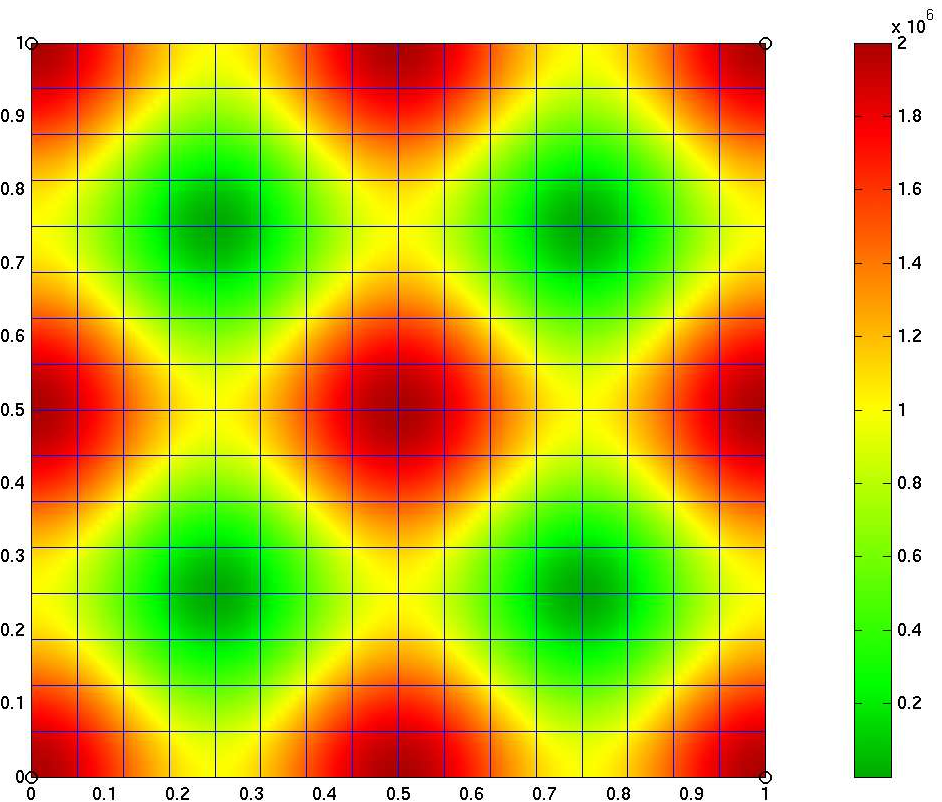
\includegraphics[width=0.45\textwidth]{figs/box}
	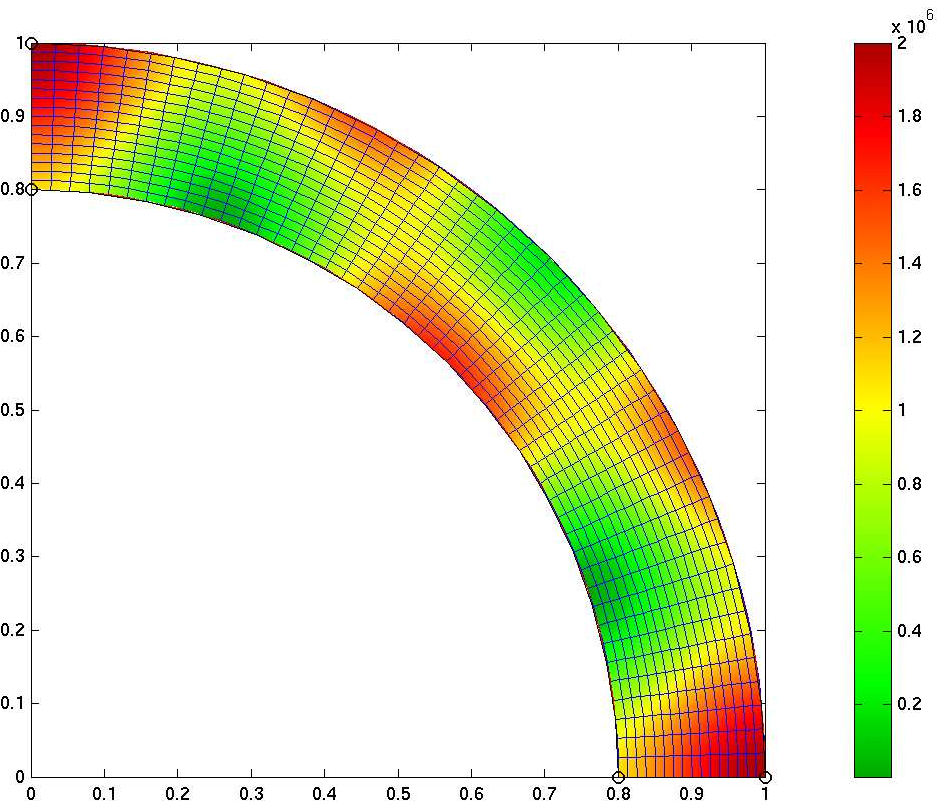
\includegraphics[width=0.45\textwidth]{figs/fan}
	\caption{\label{fig:mesh2d} The 2D meshes used for the tests.}
\end{figure}

\begin{figure}
	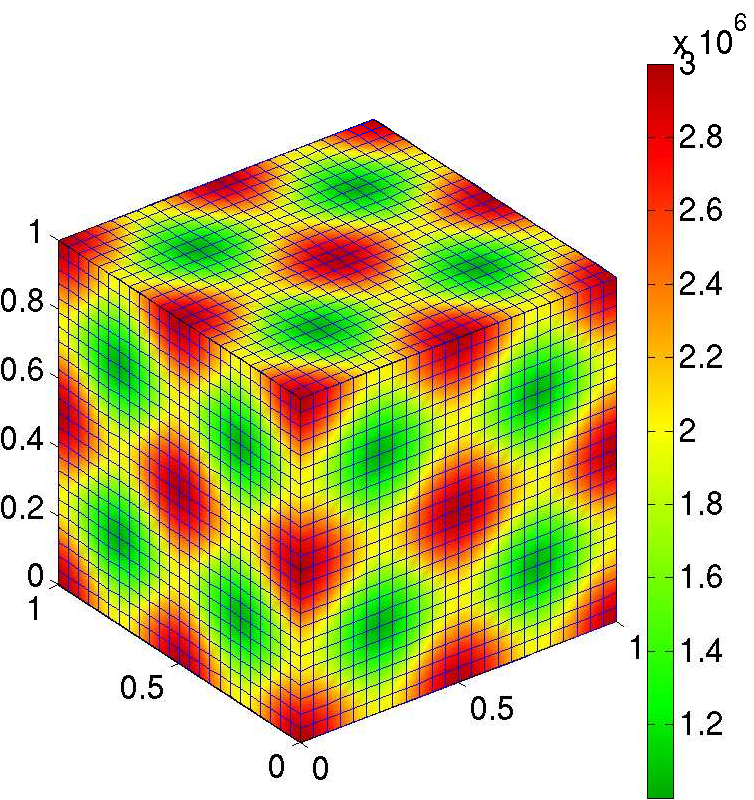
\includegraphics[width=0.45\textwidth]{figs/box3a}
	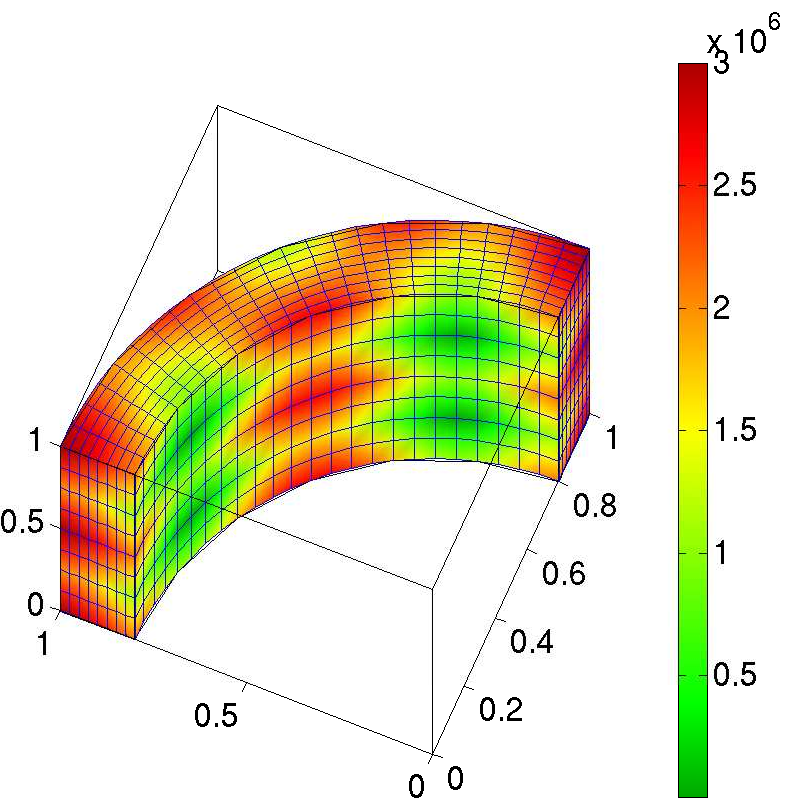
\includegraphics[width=0.45\textwidth]{figs/fan3a}
	\caption{\label{fig:mesh3d} The 3D meshes used for the tests.}
\end{figure}


\subsection{Smoothers}

\begin{figure}
	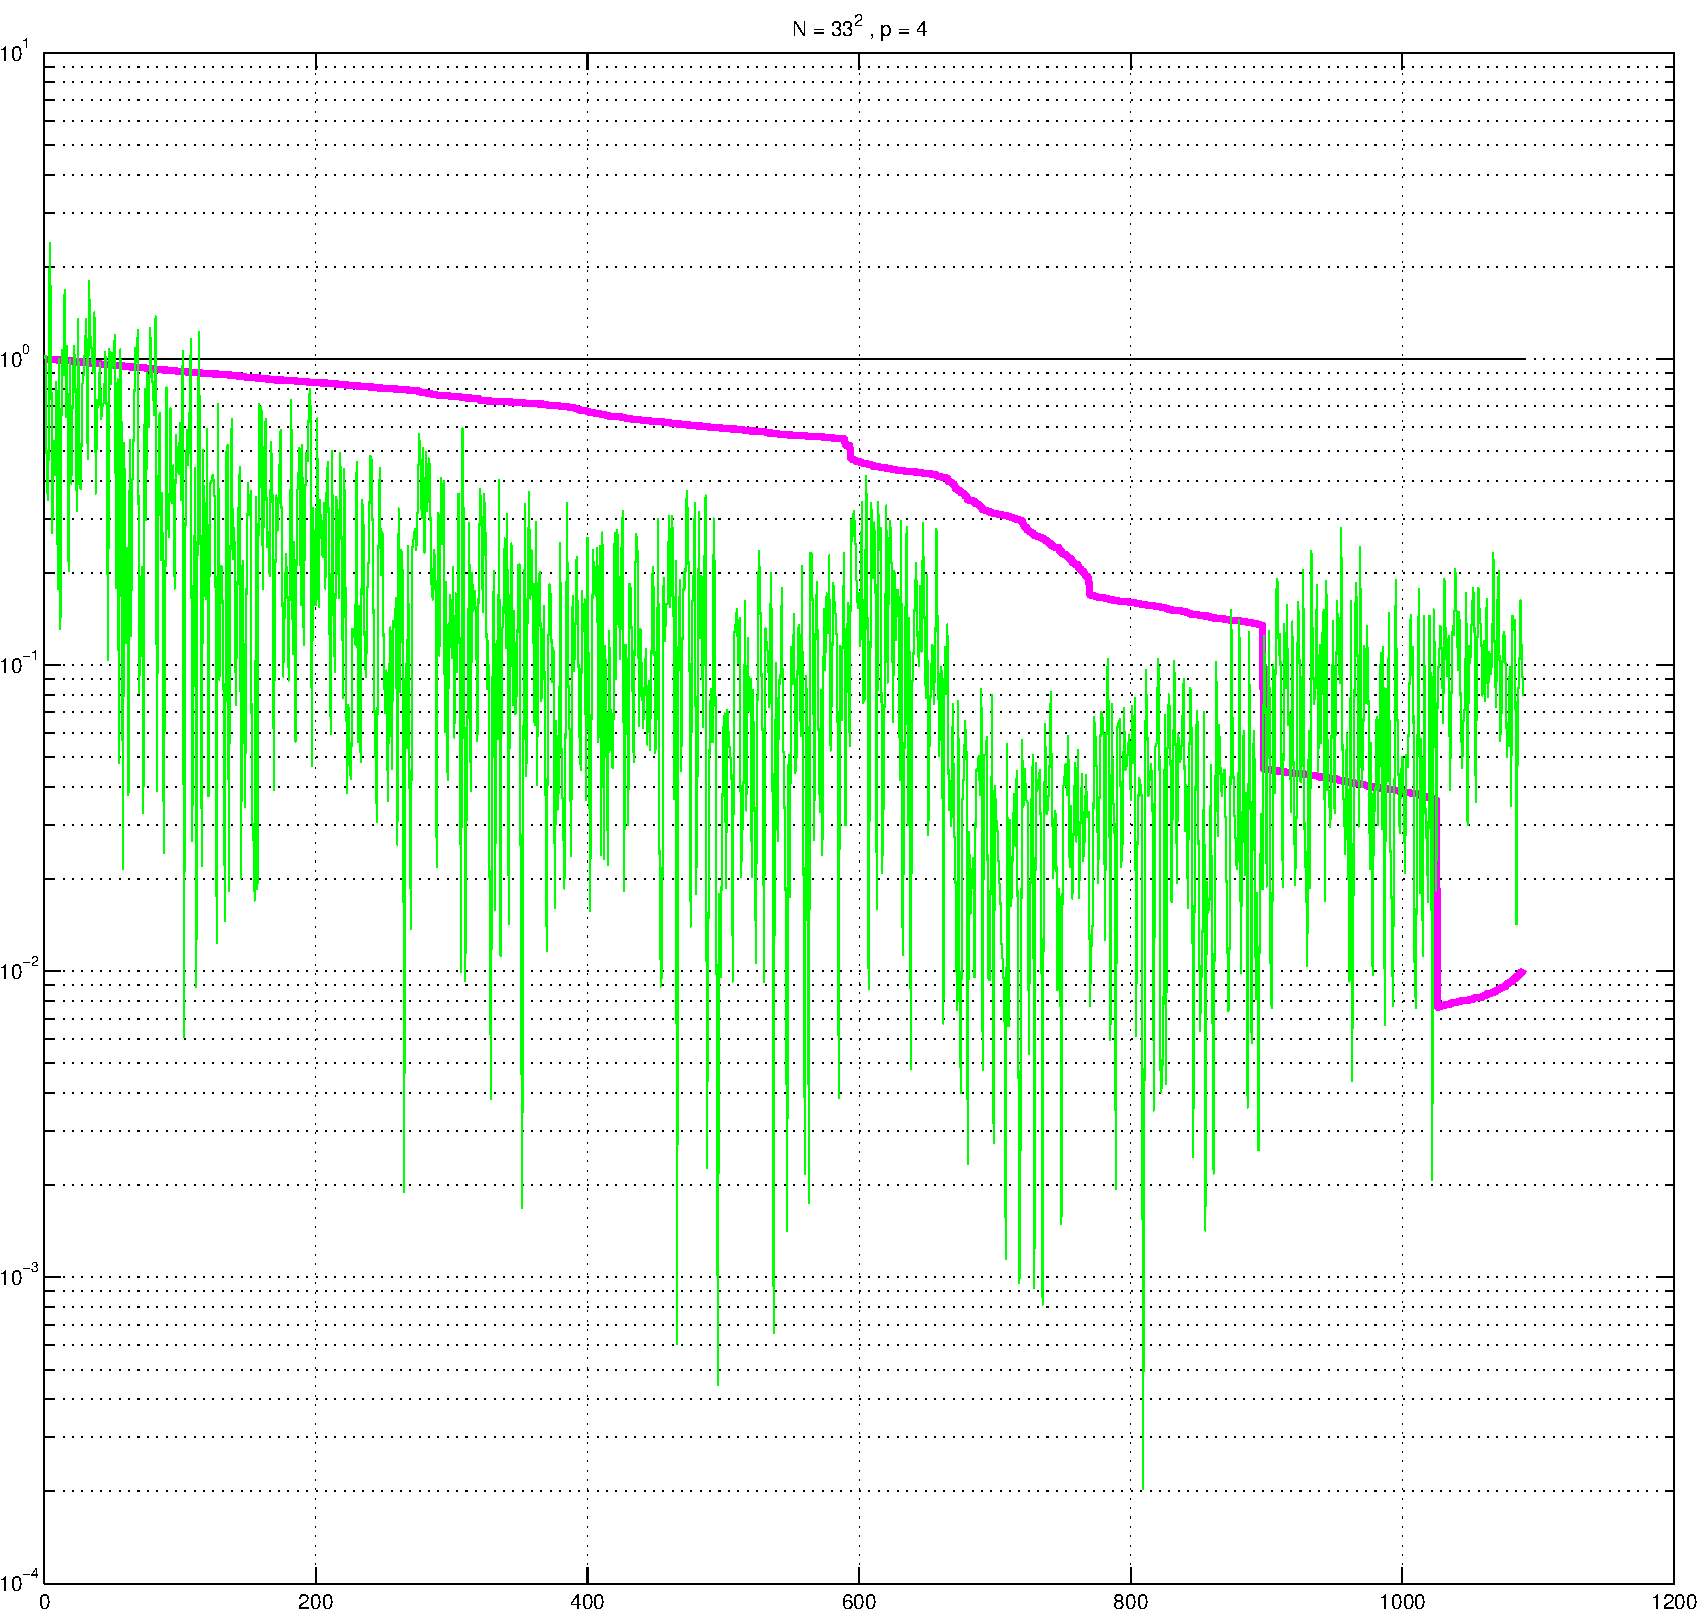
\includegraphics[width=0.45\textwidth]{figs/smoothers-order4}
	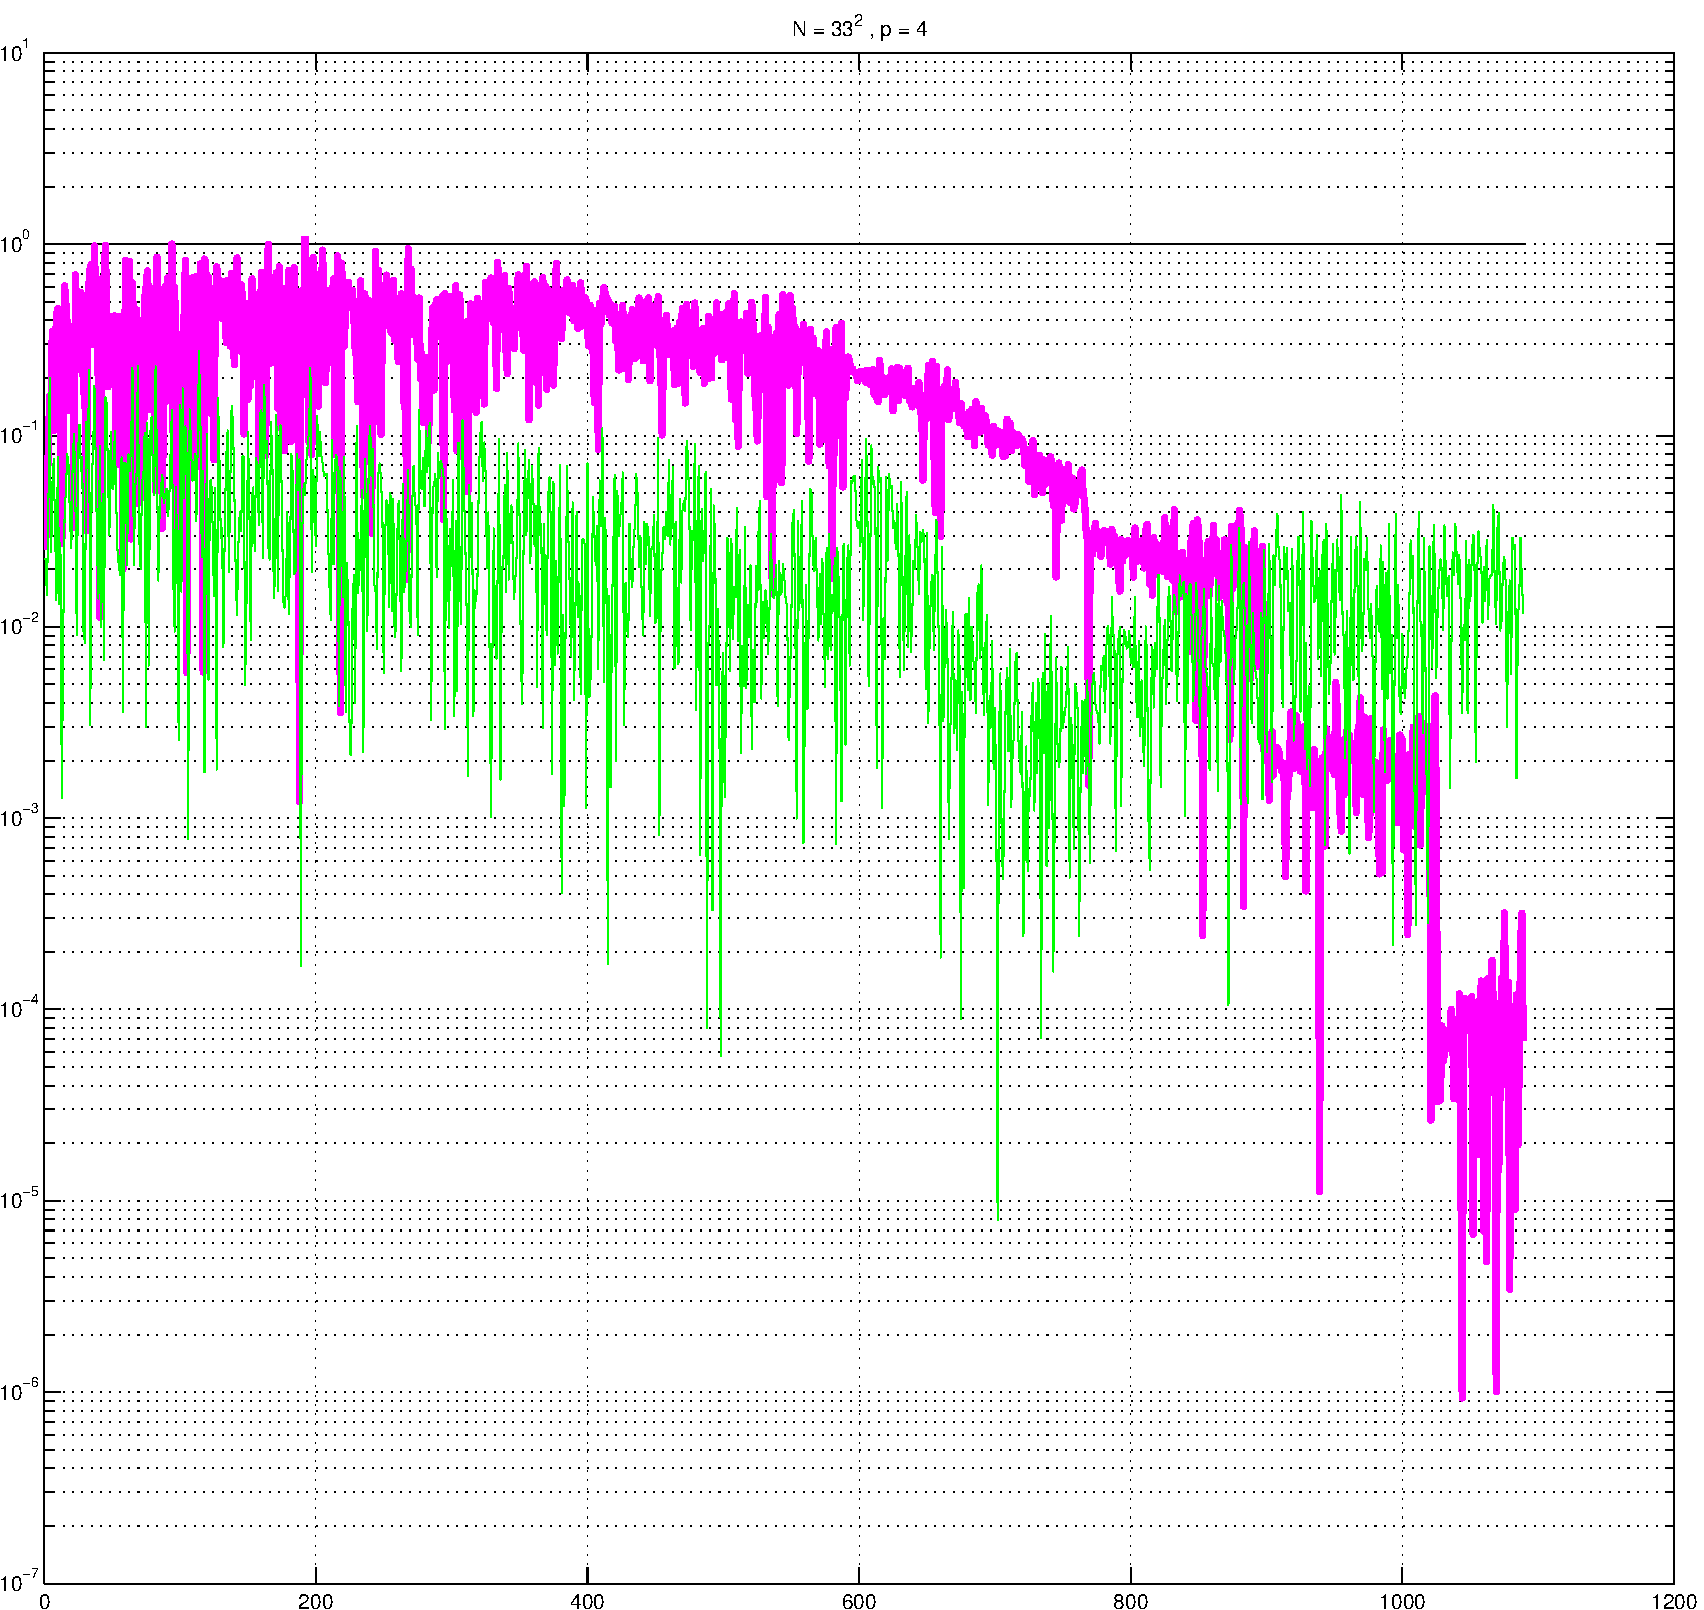
\includegraphics[width=0.45\textwidth]{figs/vcycle-order4}
	\caption{\label{fig:smoothers} The smoothing properties of the smoothers.}
\end{figure}

\begin{figure}
	% 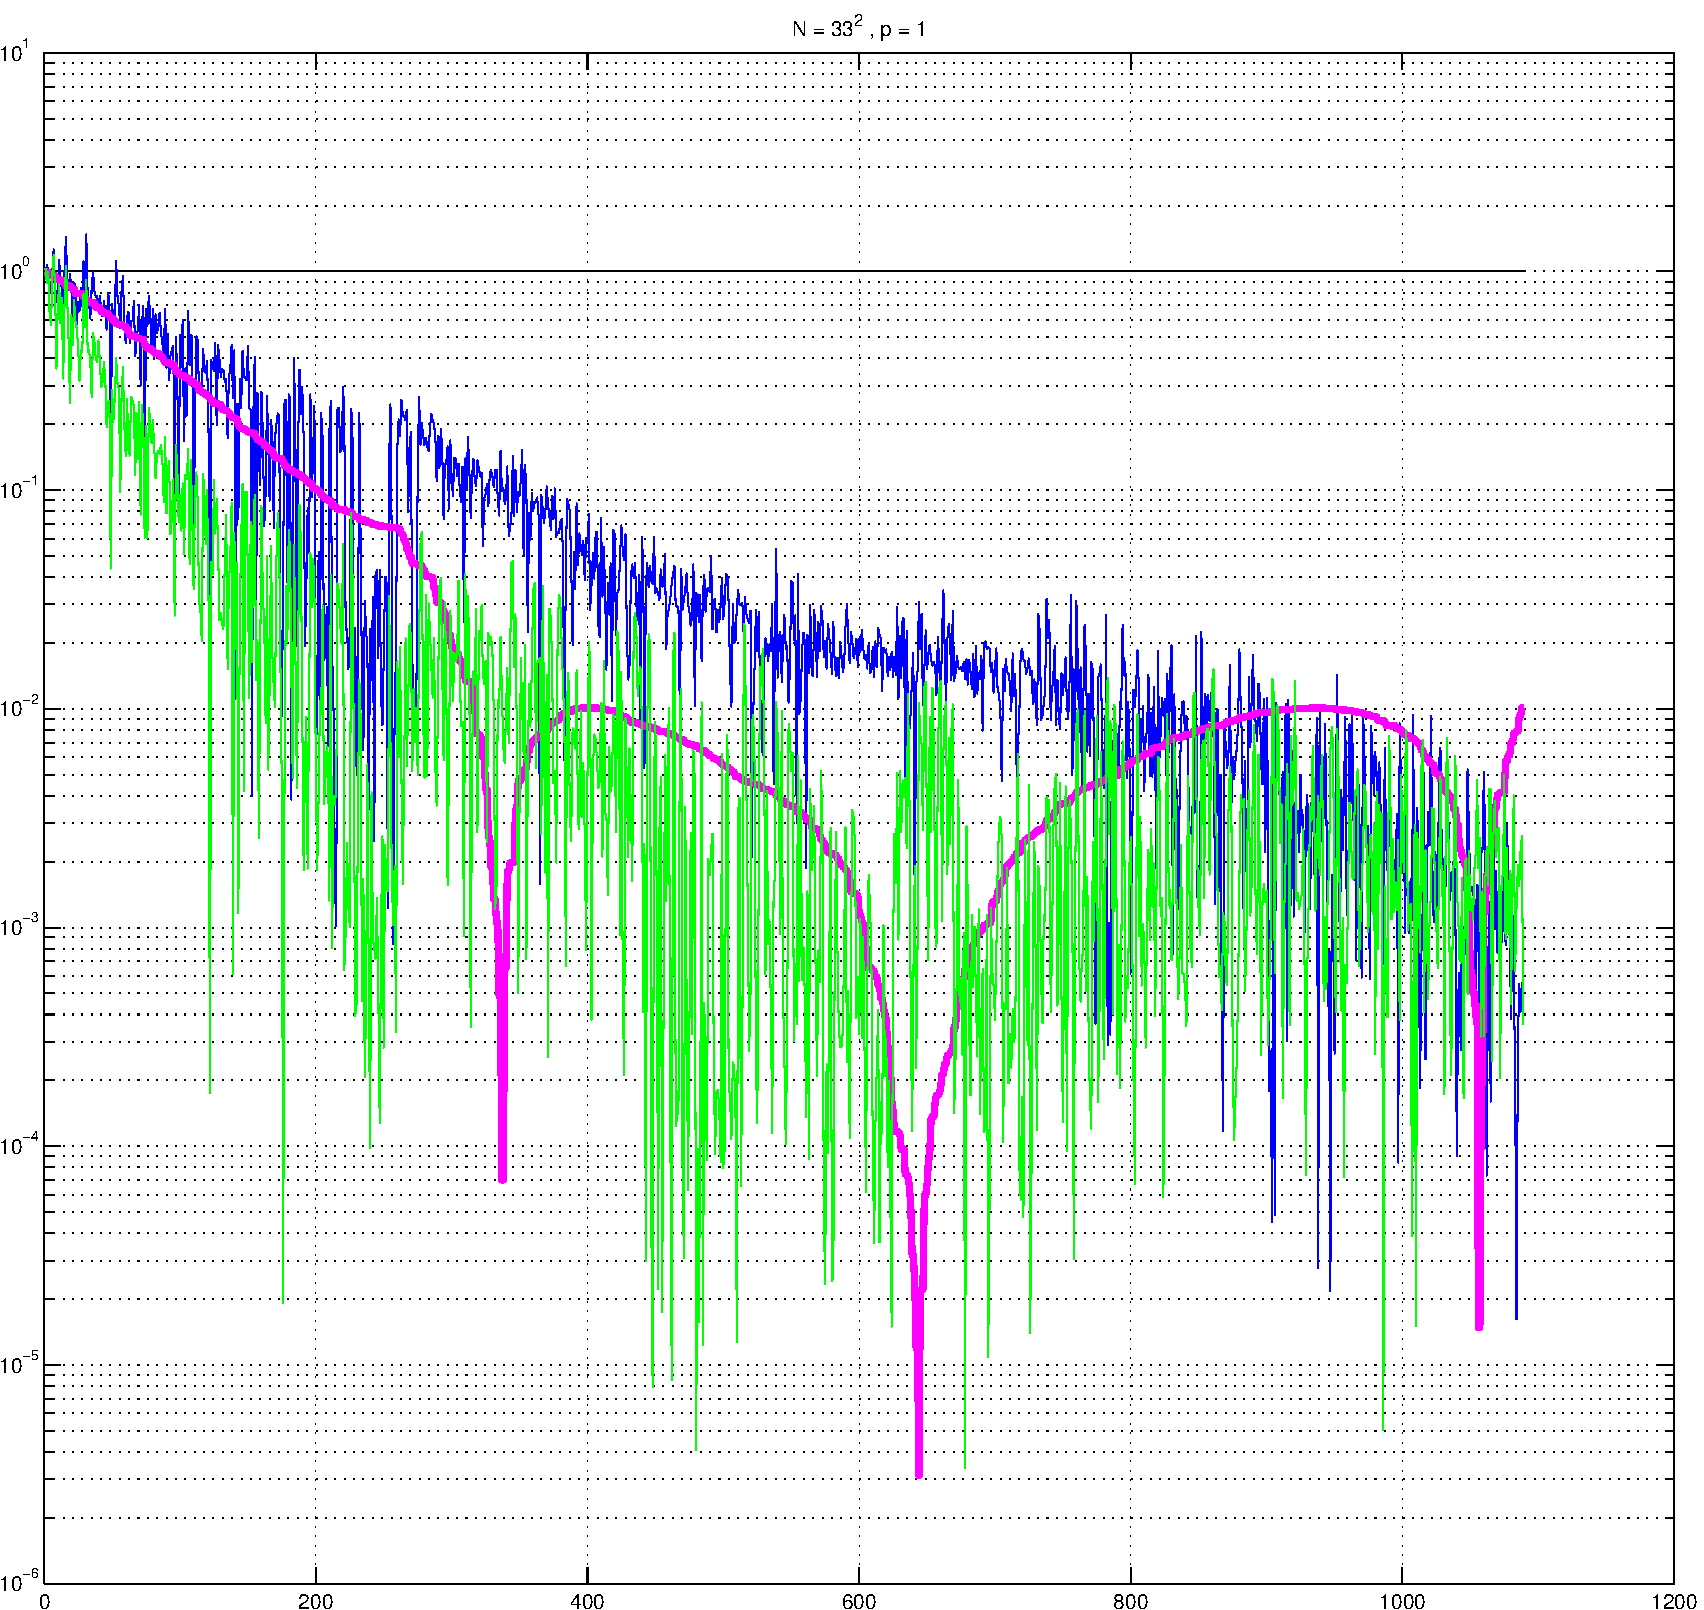
\includegraphics[width=0.45\textwidth]{figs/smoothers-order1}
	% 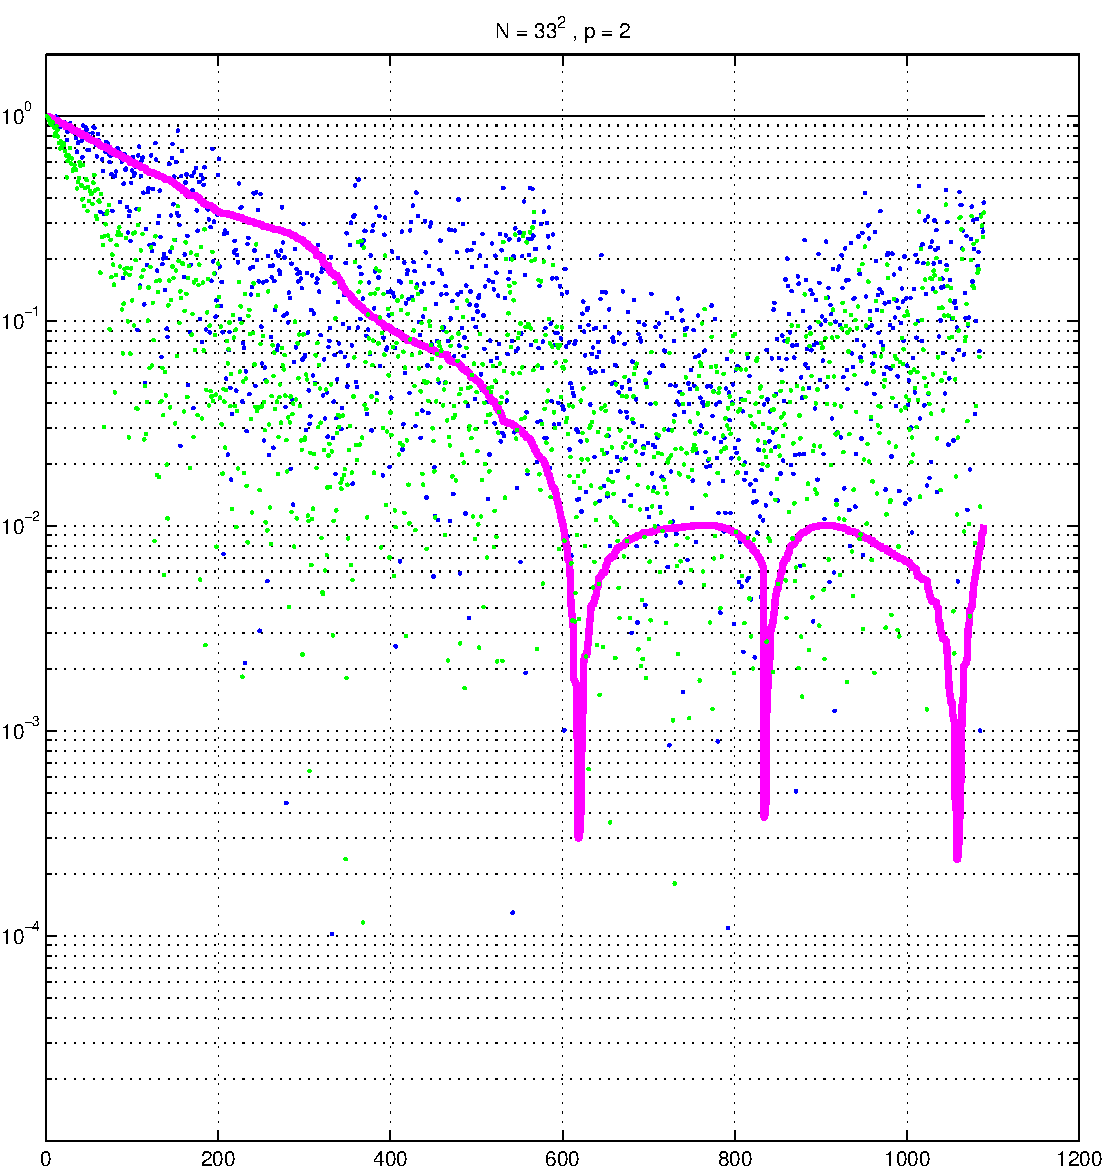
\includegraphics[width=0.45\textwidth]{figs/smoothers-order2}
	% This file was created by matlab2tikz v0.3.3.
% Copyright (c) 2008--2013, Nico Schlmer <nico.schloemer@gmail.com>
% All rights reserved.
% 
% The latest updates can be retrieved from
%   http://www.mathworks.com/matlabcentral/fileexchange/22022-matlab2tikz
% where you can also make suggestions and rate matlab2tikz.
% 
% 
% 

% defining custom colors
\definecolor{mycolor1}{rgb}{1,0,1}

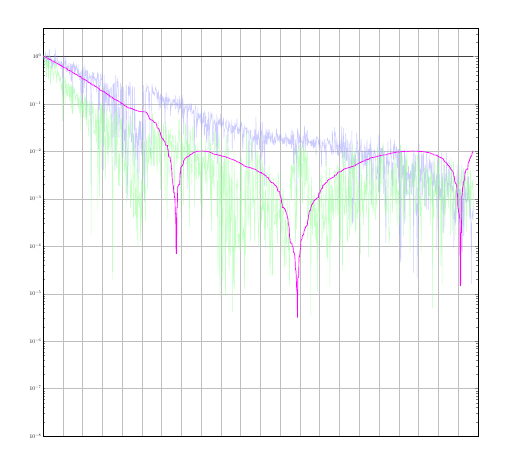
\begin{tikzpicture}[scale=0.2]

\begin{axis}[%
width=10.8672222222222in,
height=10.2056111111111in,
scale only axis,
xmin=0,
xmax=1100,
xmajorgrids,
xmajorticks=false,
ymode=log,
ymin=1e-08,
ymax=4,
% yminorticks=false,
ymajorgrids,
% yminorgrids,
% title={$\text{N = 33}^\text{2}\text{ , p = 1}$}
]
\addplot [
color=black,
solid,thick,
forget plot
]
table[row sep=crcr]{
1 1.00000000000001\\
2 0.999999999999995\\
3 0.999999999999993\\
4 1\\
5 1.00000000000001\\
6 1\\
7 1\\
8 1\\
9 1\\
10 1\\
11 0.999999999999993\\
12 0.999999999999996\\
13 0.999999999999989\\
14 0.999999999999997\\
15 0.999999999999997\\
16 1\\
17 1.00000000000001\\
18 1\\
19 1\\
20 1\\
21 1\\
22 0.999999999999994\\
23 1\\
24 1\\
25 0.999999999999998\\
26 1.00000000000001\\
27 1\\
28 1\\
29 1.00000000000001\\
30 1\\
31 0.999999999999997\\
32 1.00000000000001\\
33 0.999999999999999\\
34 1\\
35 1\\
36 0.999999999999998\\
37 0.999999999999999\\
38 1.00000000000001\\
39 1.00000000000001\\
40 0.999999999999998\\
41 1\\
42 0.999999999999996\\
43 0.999999999999987\\
44 1\\
45 1\\
46 1.00000000000001\\
47 0.999999999999997\\
48 1\\
49 1\\
50 0.999999999999999\\
51 0.999999999999993\\
52 0.999999999999997\\
53 1\\
54 1\\
55 0.999999999999994\\
56 0.999999999999999\\
57 1\\
58 1\\
59 1\\
60 0.999999999999999\\
61 1.00000000000001\\
62 1\\
63 0.999999999999999\\
64 0.999999999999997\\
65 1\\
66 0.99999999999999\\
67 1\\
68 0.999999999999994\\
69 1\\
70 0.999999999999993\\
71 0.999999999999995\\
72 1.00000000000001\\
73 0.999999999999997\\
74 1\\
75 1\\
76 1.00000000000001\\
77 1\\
78 1\\
79 1\\
80 0.999999999999996\\
81 1\\
82 1\\
83 1\\
84 1\\
85 0.999999999999998\\
86 0.999999999999996\\
87 1\\
88 0.999999999999999\\
89 0.999999999999997\\
90 1.00000000000001\\
91 1\\
92 0.999999999999995\\
93 1.00000000000001\\
94 1\\
95 0.999999999999991\\
96 1\\
97 1\\
98 1\\
99 0.999999999999991\\
100 1\\
101 1.00000000000001\\
102 1\\
103 0.99999999999999\\
104 0.999999999999999\\
105 1\\
106 0.999999999999999\\
107 1.00000000000001\\
108 1\\
109 0.99999999999999\\
110 0.99999999999999\\
111 1.00000000000001\\
112 0.999999999999999\\
113 1.00000000000001\\
114 0.999999999999994\\
115 0.999999999999996\\
116 0.999999999999992\\
117 1\\
118 1.00000000000001\\
119 0.999999999999998\\
120 0.999999999999995\\
121 1\\
122 1\\
123 1\\
124 0.999999999999998\\
125 1.00000000000001\\
126 0.999999999999999\\
127 0.999999999999992\\
128 0.999999999999999\\
129 1\\
130 0.999999999999999\\
131 1.00000000000001\\
132 0.999999999999985\\
133 0.999999999999994\\
134 1.00000000000001\\
135 0.999999999999996\\
136 1.00000000000001\\
137 1\\
138 0.999999999999994\\
139 1\\
140 0.999999999999984\\
141 1\\
142 0.999999999999998\\
143 0.999999999999999\\
144 1.00000000000001\\
145 1.00000000000001\\
146 1\\
147 0.999999999999995\\
148 0.999999999999995\\
149 1.00000000000001\\
150 0.999999999999996\\
151 1\\
152 0.999999999999999\\
153 1.00000000000001\\
154 1\\
155 0.999999999999991\\
156 0.999999999999996\\
157 1\\
158 1.00000000000001\\
159 0.999999999999995\\
160 1\\
161 0.999999999999992\\
162 0.999999999999993\\
163 1\\
164 0.999999999999999\\
165 0.999999999999995\\
166 0.999999999999998\\
167 0.999999999999994\\
168 0.999999999999997\\
169 0.999999999999999\\
170 0.999999999999992\\
171 0.999999999999996\\
172 1\\
173 1.00000000000001\\
174 1.00000000000001\\
175 1\\
176 1\\
177 1.00000000000001\\
178 0.999999999999997\\
179 1\\
180 1.00000000000002\\
181 1.00000000000001\\
182 1\\
183 1.00000000000001\\
184 0.999999999999995\\
185 0.999999999999993\\
186 0.999999999999998\\
187 0.999999999999993\\
188 1\\
189 1\\
190 1.00000000000001\\
191 0.999999999999994\\
192 1\\
193 1\\
194 1\\
195 0.999999999999998\\
196 1\\
197 0.999999999999999\\
198 1\\
199 1\\
200 1\\
201 0.999999999999995\\
202 1\\
203 1.00000000000001\\
204 1\\
205 1\\
206 0.999999999999991\\
207 1\\
208 0.999999999999996\\
209 0.999999999999998\\
210 0.999999999999998\\
211 0.999999999999998\\
212 1.00000000000001\\
213 1\\
214 0.999999999999997\\
215 0.999999999999988\\
216 1\\
217 1\\
218 1.00000000000001\\
219 1.00000000000001\\
220 0.999999999999991\\
221 0.999999999999996\\
222 0.99999999999999\\
223 0.999999999999997\\
224 0.999999999999997\\
225 0.999999999999999\\
226 0.999999999999998\\
227 0.999999999999986\\
228 1\\
229 0.999999999999997\\
230 0.999999999999997\\
231 0.999999999999983\\
232 0.999999999999995\\
233 1.00000000000001\\
234 0.999999999999997\\
235 0.999999999999996\\
236 0.999999999999999\\
237 0.999999999999988\\
238 1\\
239 0.999999999999998\\
240 0.99999999999999\\
241 1\\
242 0.999999999999986\\
243 0.999999999999996\\
244 1\\
245 0.999999999999993\\
246 1\\
247 1.00000000000001\\
248 1\\
249 0.999999999999994\\
250 1\\
251 1\\
252 0.999999999999995\\
253 0.999999999999995\\
254 1.00000000000001\\
255 0.999999999999997\\
256 0.999999999999997\\
257 1\\
258 1\\
259 0.999999999999996\\
260 0.999999999999995\\
261 1.00000000000001\\
262 1.00000000000001\\
263 0.999999999999994\\
264 1.00000000000001\\
265 1\\
266 1.00000000000001\\
267 0.999999999999995\\
268 0.999999999999999\\
269 1\\
270 1.00000000000001\\
271 1\\
272 0.999999999999998\\
273 0.999999999999999\\
274 1\\
275 1.00000000000001\\
276 0.999999999999999\\
277 0.999999999999998\\
278 1.00000000000001\\
279 1.00000000000001\\
280 0.999999999999996\\
281 0.99999999999999\\
282 1\\
283 1\\
284 0.999999999999998\\
285 1.00000000000001\\
286 0.999999999999993\\
287 1.00000000000001\\
288 1\\
289 0.999999999999992\\
290 0.999999999999995\\
291 1.00000000000001\\
292 0.999999999999999\\
293 0.999999999999996\\
294 0.999999999999989\\
295 1.00000000000001\\
296 0.999999999999988\\
297 0.999999999999996\\
298 0.999999999999997\\
299 0.999999999999998\\
300 1\\
301 1.00000000000001\\
302 1\\
303 0.999999999999999\\
304 1\\
305 0.999999999999992\\
306 0.999999999999996\\
307 1\\
308 0.999999999999996\\
309 1\\
310 1\\
311 0.99999999999999\\
312 1\\
313 1\\
314 1\\
315 1.00000000000001\\
316 0.999999999999993\\
317 0.999999999999991\\
318 1.00000000000001\\
319 0.999999999999983\\
320 1.00000000000002\\
321 0.999999999999994\\
322 0.999999999999992\\
323 0.99999999999999\\
324 1.00000000000001\\
325 1\\
326 1\\
327 1.00000000000001\\
328 0.999999999999997\\
329 0.999999999999982\\
330 1\\
331 0.999999999999995\\
332 0.999999999999993\\
333 0.999999999999997\\
334 0.999999999999999\\
335 0.999999999999997\\
336 1.00000000000001\\
337 0.999999999999986\\
338 1\\
339 1.00000000000001\\
340 0.999999999999987\\
341 0.999999999999993\\
342 0.999999999999997\\
343 0.999999999999999\\
344 1.00000000000001\\
345 1\\
346 0.999999999999999\\
347 0.999999999999997\\
348 1\\
349 1.00000000000001\\
350 0.999999999999995\\
351 1\\
352 0.999999999999994\\
353 0.999999999999989\\
354 0.999999999999996\\
355 0.999999999999996\\
356 1.00000000000001\\
357 0.999999999999999\\
358 0.999999999999999\\
359 1.00000000000001\\
360 1\\
361 0.999999999999997\\
362 0.999999999999992\\
363 0.999999999999994\\
364 1.00000000000001\\
365 1.00000000000001\\
366 1.00000000000001\\
367 0.999999999999996\\
368 1\\
369 1.00000000000001\\
370 1\\
371 0.999999999999992\\
372 1\\
373 1\\
374 1.00000000000001\\
375 1\\
376 0.999999999999993\\
377 0.999999999999996\\
378 1\\
379 0.999999999999991\\
380 0.999999999999995\\
381 0.999999999999992\\
382 1\\
383 1\\
384 0.999999999999985\\
385 0.999999999999999\\
386 1.00000000000001\\
387 1.00000000000001\\
388 1.00000000000001\\
389 0.999999999999992\\
390 1\\
391 1\\
392 0.999999999999997\\
393 0.999999999999988\\
394 0.999999999999984\\
395 1.00000000000001\\
396 1\\
397 1.00000000000001\\
398 0.999999999999997\\
399 0.999999999999994\\
400 1\\
401 1\\
402 0.999999999999993\\
403 1\\
404 0.999999999999997\\
405 1\\
406 1.00000000000001\\
407 0.999999999999994\\
408 1.00000000000001\\
409 0.999999999999992\\
410 1\\
411 0.999999999999999\\
412 1\\
413 0.999999999999989\\
414 0.999999999999996\\
415 0.999999999999997\\
416 1.00000000000001\\
417 0.999999999999996\\
418 1.00000000000001\\
419 1\\
420 1\\
421 1\\
422 0.999999999999985\\
423 1.00000000000001\\
424 0.999999999999996\\
425 0.999999999999995\\
426 0.99999999999999\\
427 0.999999999999999\\
428 0.999999999999989\\
429 1\\
430 0.999999999999996\\
431 0.999999999999988\\
432 0.999999999999991\\
433 0.999999999999986\\
434 1\\
435 1.00000000000001\\
436 0.999999999999998\\
437 0.999999999999997\\
438 1\\
439 0.999999999999996\\
440 0.999999999999994\\
441 0.999999999999997\\
442 0.999999999999989\\
443 0.999999999999988\\
444 1\\
445 1\\
446 0.99999999999999\\
447 1\\
448 1\\
449 1\\
450 0.999999999999998\\
451 0.999999999999991\\
452 0.999999999999991\\
453 1.00000000000001\\
454 0.999999999999989\\
455 0.999999999999988\\
456 1.00000000000001\\
457 1.00000000000001\\
458 1\\
459 0.999999999999994\\
460 1.00000000000001\\
461 1\\
462 1\\
463 1\\
464 0.999999999999998\\
465 1\\
466 0.999999999999978\\
467 1\\
468 0.999999999999998\\
469 1\\
470 1\\
471 0.999999999999998\\
472 0.999999999999993\\
473 1\\
474 0.999999999999999\\
475 1.00000000000001\\
476 0.999999999999981\\
477 0.999999999999999\\
478 0.999999999999999\\
479 1\\
480 0.999999999999992\\
481 1\\
482 1\\
483 0.999999999999993\\
484 1\\
485 1.00000000000001\\
486 0.999999999999999\\
487 0.999999999999994\\
488 0.999999999999996\\
489 1\\
490 0.999999999999996\\
491 1\\
492 1\\
493 0.999999999999992\\
494 0.999999999999993\\
495 1.00000000000001\\
496 0.999999999999996\\
497 0.999999999999994\\
498 1\\
499 0.999999999999989\\
500 1\\
501 1\\
502 0.99999999999999\\
503 1\\
504 1\\
505 1.00000000000001\\
506 1\\
507 1.00000000000001\\
508 0.999999999999995\\
509 1.00000000000001\\
510 0.999999999999996\\
511 1\\
512 0.999999999999994\\
513 0.999999999999992\\
514 1\\
515 1\\
516 1\\
517 0.999999999999995\\
518 0.999999999999983\\
519 0.99999999999999\\
520 0.999999999999993\\
521 1.00000000000001\\
522 0.999999999999999\\
523 1.00000000000001\\
524 1.00000000000001\\
525 0.999999999999999\\
526 1\\
527 1\\
528 0.999999999999999\\
529 1\\
530 0.999999999999996\\
531 0.999999999999996\\
532 0.999999999999994\\
533 1.00000000000001\\
534 0.999999999999995\\
535 1\\
536 1\\
537 1.00000000000001\\
538 0.999999999999987\\
539 0.999999999999995\\
540 0.999999999999994\\
541 1\\
542 0.999999999999991\\
543 0.999999999999995\\
544 0.999999999999995\\
545 0.999999999999988\\
546 1\\
547 0.999999999999989\\
548 0.99999999999999\\
549 0.999999999999995\\
550 0.999999999999993\\
551 0.999999999999993\\
552 0.99999999999999\\
553 1\\
554 1\\
555 0.999999999999986\\
556 1\\
557 1.00000000000001\\
558 0.999999999999994\\
559 1.00000000000001\\
560 0.999999999999986\\
561 1\\
562 1.00000000000001\\
563 1\\
564 0.999999999999994\\
565 0.999999999999998\\
566 0.999999999999987\\
567 1\\
568 0.999999999999999\\
569 1.00000000000001\\
570 0.999999999999986\\
571 1\\
572 0.999999999999995\\
573 1\\
574 1.00000000000001\\
575 1.00000000000001\\
576 0.999999999999987\\
577 0.999999999999999\\
578 0.999999999999996\\
579 1\\
580 0.999999999999996\\
581 1\\
582 1\\
583 0.999999999999983\\
584 0.999999999999992\\
585 1.00000000000001\\
586 1\\
587 0.999999999999999\\
588 1.00000000000001\\
589 1.00000000000001\\
590 0.999999999999997\\
591 0.999999999999996\\
592 1\\
593 0.999999999999998\\
594 0.999999999999991\\
595 0.999999999999996\\
596 1\\
597 1.00000000000001\\
598 1.00000000000001\\
599 0.999999999999998\\
600 0.999999999999995\\
601 1.00000000000001\\
602 0.999999999999998\\
603 0.999999999999998\\
604 0.999999999999999\\
605 0.999999999999997\\
606 1.00000000000001\\
607 0.999999999999992\\
608 1.00000000000001\\
609 1\\
610 0.99999999999999\\
611 1.00000000000001\\
612 1\\
613 0.999999999999999\\
614 0.999999999999994\\
615 1.00000000000001\\
616 0.999999999999999\\
617 0.999999999999998\\
618 1\\
619 0.999999999999995\\
620 1.00000000000001\\
621 0.999999999999996\\
622 1\\
623 1.00000000000001\\
624 1\\
625 1\\
626 1.00000000000001\\
627 0.99999999999999\\
628 0.999999999999986\\
629 0.999999999999991\\
630 0.999999999999997\\
631 1.00000000000001\\
632 1\\
633 1.00000000000002\\
634 0.999999999999998\\
635 0.999999999999996\\
636 1\\
637 0.999999999999984\\
638 1.00000000000001\\
639 0.999999999999998\\
640 1\\
641 1.00000000000003\\
642 1.00000000000001\\
643 1\\
644 0.999999999999995\\
645 0.999999999999976\\
646 1\\
647 0.999999999999994\\
648 1.00000000000001\\
649 1.00000000000001\\
650 0.999999999999992\\
651 1\\
652 1\\
653 0.999999999999997\\
654 0.999999999999992\\
655 0.999999999999998\\
656 1.00000000000001\\
657 0.999999999999992\\
658 0.999999999999984\\
659 1.00000000000002\\
660 1\\
661 1\\
662 0.99999999999999\\
663 1\\
664 0.999999999999996\\
665 1\\
666 1.00000000000001\\
667 0.999999999999997\\
668 1.00000000000001\\
669 1\\
670 1\\
671 0.999999999999994\\
672 0.999999999999989\\
673 0.999999999999995\\
674 0.999999999999993\\
675 0.999999999999998\\
676 0.999999999999998\\
677 1.00000000000001\\
678 0.999999999999994\\
679 1.00000000000001\\
680 1\\
681 0.999999999999983\\
682 1\\
683 1.00000000000001\\
684 0.999999999999988\\
685 1\\
686 1\\
687 0.999999999999988\\
688 0.999999999999991\\
689 0.999999999999995\\
690 1.00000000000001\\
691 1.00000000000001\\
692 1.00000000000001\\
693 1.00000000000001\\
694 0.999999999999999\\
695 1\\
696 1\\
697 1\\
698 1.00000000000001\\
699 1.00000000000001\\
700 0.999999999999998\\
701 1\\
702 0.999999999999987\\
703 1\\
704 0.999999999999982\\
705 1\\
706 1\\
707 0.999999999999986\\
708 1.00000000000001\\
709 0.999999999999995\\
710 0.999999999999998\\
711 1\\
712 0.999999999999991\\
713 1\\
714 0.999999999999991\\
715 0.999999999999993\\
716 1.00000000000001\\
717 1\\
718 0.999999999999987\\
719 0.999999999999992\\
720 1.00000000000001\\
721 0.999999999999993\\
722 1.00000000000001\\
723 1\\
724 0.999999999999996\\
725 1\\
726 1\\
727 1.00000000000001\\
728 1.00000000000001\\
729 1.00000000000001\\
730 0.999999999999996\\
731 1.00000000000002\\
732 0.999999999999992\\
733 1\\
734 0.999999999999986\\
735 0.999999999999991\\
736 1.00000000000001\\
737 1.00000000000001\\
738 1.00000000000001\\
739 0.999999999999993\\
740 1\\
741 1.00000000000002\\
742 0.999999999999989\\
743 0.999999999999998\\
744 1\\
745 1\\
746 1.00000000000002\\
747 0.999999999999997\\
748 1\\
749 1\\
750 0.999999999999999\\
751 0.999999999999994\\
752 1\\
753 0.999999999999995\\
754 0.999999999999996\\
755 1.00000000000001\\
756 0.999999999999992\\
757 1.00000000000001\\
758 1.00000000000001\\
759 1.00000000000001\\
760 0.999999999999999\\
761 1.00000000000002\\
762 0.999999999999996\\
763 1\\
764 0.99999999999999\\
765 1.00000000000001\\
766 0.999999999999978\\
767 0.999999999999993\\
768 0.999999999999997\\
769 0.999999999999993\\
770 1\\
771 0.999999999999993\\
772 0.99999999999999\\
773 1.00000000000002\\
774 1.00000000000002\\
775 1\\
776 0.999999999999989\\
777 1.00000000000001\\
778 1\\
779 0.999999999999981\\
780 1\\
781 0.999999999999985\\
782 1.00000000000001\\
783 1\\
784 0.999999999999986\\
785 0.999999999999988\\
786 0.999999999999988\\
787 1.00000000000001\\
788 1.00000000000002\\
789 1\\
790 1\\
791 1.00000000000001\\
792 0.999999999999995\\
793 1.00000000000002\\
794 1.00000000000001\\
795 0.999999999999996\\
796 0.999999999999979\\
797 0.999999999999994\\
798 0.999999999999999\\
799 1.00000000000001\\
800 0.999999999999997\\
801 0.99999999999998\\
802 1.00000000000001\\
803 0.999999999999997\\
804 0.999999999999985\\
805 0.99999999999999\\
806 1\\
807 1.00000000000001\\
808 1.00000000000001\\
809 1\\
810 0.99999999999998\\
811 0.999999999999987\\
812 1.00000000000001\\
813 0.999999999999995\\
814 1.00000000000001\\
815 0.999999999999995\\
816 0.99999999999998\\
817 0.999999999999997\\
818 1.00000000000001\\
819 0.999999999999996\\
820 0.99999999999999\\
821 0.999999999999992\\
822 0.999999999999989\\
823 0.999999999999997\\
824 0.999999999999994\\
825 0.999999999999979\\
826 1.00000000000001\\
827 0.999999999999999\\
828 1.00000000000001\\
829 1.00000000000001\\
830 0.999999999999999\\
831 0.999999999999998\\
832 0.999999999999998\\
833 1.00000000000001\\
834 1\\
835 1.00000000000001\\
836 1\\
837 0.999999999999996\\
838 0.999999999999997\\
839 0.999999999999995\\
840 1.00000000000001\\
841 0.999999999999995\\
842 1\\
843 1.00000000000001\\
844 0.999999999999992\\
845 1\\
846 1\\
847 0.999999999999981\\
848 0.999999999999989\\
849 1.00000000000002\\
850 1.00000000000001\\
851 1\\
852 0.999999999999995\\
853 1\\
854 0.999999999999991\\
855 0.999999999999991\\
856 0.999999999999992\\
857 1.00000000000001\\
858 1.00000000000002\\
859 0.999999999999994\\
860 1.00000000000001\\
861 0.999999999999992\\
862 0.999999999999996\\
863 1\\
864 0.999999999999998\\
865 0.999999999999999\\
866 0.999999999999999\\
867 0.999999999999993\\
868 1\\
869 1\\
870 1.00000000000001\\
871 0.999999999999995\\
872 0.999999999999986\\
873 1\\
874 1.00000000000001\\
875 0.999999999999992\\
876 1.00000000000001\\
877 0.999999999999997\\
878 1\\
879 1.00000000000001\\
880 1\\
881 1.00000000000001\\
882 1\\
883 1.00000000000001\\
884 0.999999999999992\\
885 0.999999999999998\\
886 1.00000000000002\\
887 1.00000000000001\\
888 0.999999999999992\\
889 0.99999999999999\\
890 0.999999999999995\\
891 1.00000000000002\\
892 0.999999999999993\\
893 0.999999999999998\\
894 1.00000000000001\\
895 0.99999999999999\\
896 0.999999999999995\\
897 1.00000000000002\\
898 0.999999999999999\\
899 0.999999999999996\\
900 1.00000000000001\\
901 1\\
902 0.999999999999999\\
903 0.999999999999996\\
904 1.00000000000001\\
905 1.00000000000001\\
906 0.999999999999998\\
907 1.00000000000001\\
908 0.999999999999996\\
909 1\\
910 0.999999999999998\\
911 0.999999999999992\\
912 1\\
913 0.99999999999999\\
914 0.999999999999981\\
915 1\\
916 1.00000000000001\\
917 1\\
918 1\\
919 1.00000000000001\\
920 0.999999999999998\\
921 0.999999999999996\\
922 0.999999999999996\\
923 0.99999999999999\\
924 0.999999999999998\\
925 1\\
926 1.00000000000002\\
927 1.00000000000001\\
928 0.999999999999985\\
929 1.00000000000001\\
930 0.999999999999981\\
931 0.999999999999975\\
932 1.00000000000001\\
933 0.999999999999993\\
934 0.99999999999999\\
935 0.999999999999993\\
936 0.999999999999982\\
937 0.999999999999997\\
938 1\\
939 0.99999999999999\\
940 0.999999999999973\\
941 1.00000000000001\\
942 0.999999999999994\\
943 0.999999999999988\\
944 0.999999999999993\\
945 1.00000000000001\\
946 1.00000000000001\\
947 1\\
948 1.00000000000001\\
949 0.999999999999998\\
950 1\\
951 0.999999999999993\\
952 1.00000000000001\\
953 1.00000000000001\\
954 0.999999999999987\\
955 0.999999999999999\\
956 1.00000000000001\\
957 1.00000000000001\\
958 1.00000000000001\\
959 0.999999999999988\\
960 1\\
961 0.999999999999991\\
962 0.999999999999991\\
963 1.00000000000001\\
964 1\\
965 0.999999999999992\\
966 0.999999999999994\\
967 1\\
968 1.00000000000002\\
969 0.999999999999991\\
970 1\\
971 0.99999999999999\\
972 0.999999999999989\\
973 0.999999999999988\\
974 0.999999999999978\\
975 0.999999999999996\\
976 0.999999999999993\\
977 0.999999999999999\\
978 1\\
979 0.99999999999999\\
980 1.00000000000001\\
981 0.999999999999992\\
982 1\\
983 1.00000000000001\\
984 0.999999999999991\\
985 1.00000000000001\\
986 1.00000000000001\\
987 1\\
988 0.999999999999985\\
989 1.00000000000001\\
990 1\\
991 0.999999999999992\\
992 0.999999999999998\\
993 1.00000000000001\\
994 0.999999999999993\\
995 0.999999999999988\\
996 0.999999999999996\\
997 0.999999999999982\\
998 0.999999999999994\\
999 1.00000000000001\\
1000 0.999999999999992\\
1001 0.999999999999989\\
1002 0.999999999999997\\
1003 1\\
1004 0.999999999999994\\
1005 1\\
1006 1\\
1007 0.999999999999998\\
1008 1\\
1009 1\\
1010 1\\
1011 1\\
1012 1.00000000000001\\
1013 1.00000000000001\\
1014 1\\
1015 1\\
1016 1.00000000000002\\
1017 1\\
1018 1.00000000000001\\
1019 1\\
1020 1\\
1021 0.999999999999999\\
1022 0.999999999999998\\
1023 1\\
1024 1\\
1025 1\\
1026 0.999999999999996\\
1027 0.999999999999998\\
1028 1.00000000000001\\
1029 1\\
1030 1\\
1031 0.999999999999997\\
1032 1\\
1033 1\\
1034 1\\
1035 1\\
1036 1.00000000000001\\
1037 0.999999999999987\\
1038 1.00000000000001\\
1039 0.999999999999994\\
1040 1.00000000000001\\
1041 1.00000000000002\\
1042 1\\
1043 1.00000000000001\\
1044 1.00000000000001\\
1045 0.999999999999985\\
1046 1\\
1047 0.999999999999997\\
1048 0.999999999999996\\
1049 0.999999999999998\\
1050 0.999999999999996\\
1051 0.999999999999999\\
1052 0.999999999999992\\
1053 1.00000000000001\\
1054 1.00000000000001\\
1055 0.999999999999999\\
1056 1.00000000000001\\
1057 0.999999999999993\\
1058 1\\
1059 0.999999999999995\\
1060 0.999999999999999\\
1061 0.999999999999989\\
1062 0.999999999999992\\
1063 1.00000000000002\\
1064 1.00000000000001\\
1065 0.999999999999988\\
1066 0.999999999999998\\
1067 1\\
1068 0.999999999999982\\
1069 1.00000000000002\\
1070 1\\
1071 1\\
1072 0.999999999999986\\
1073 0.999999999999993\\
1074 0.999999999999986\\
1075 0.999999999999999\\
1076 1.00000000000001\\
1077 1\\
1078 0.999999999999995\\
1079 1.00000000000001\\
1080 0.999999999999994\\
1081 0.999999999999988\\
1082 1\\
1083 1\\
1084 1.00000000000001\\
1085 1\\
1086 1\\
1087 1.00000000000001\\
1088 1\\
1089 1.00000000000001\\
};
\addplot [
color=blue!40,
opacity=0.5,
solid,thick,
forget plot
]
table[row sep=crcr]{
1 0.980713521202408\\
2 1.06967247781685\\
3 1.01074460777748\\
4 0.814558984908198\\
5 0.854085403861034\\
6 0.988327876449661\\
7 1.26210254083276\\
8 0.82648824045788\\
9 0.72638292820056\\
10 0.845216572596158\\
11 1.12810521673016\\
12 0.862430226969949\\
13 0.922621450678224\\
14 0.546142667861782\\
15 1.04624881081685\\
16 1.44264566335871\\
17 0.890813823018154\\
18 0.825195421810088\\
19 0.972689994034164\\
20 0.840073271031526\\
21 0.54746876881327\\
22 0.885164107054228\\
23 0.856453648178297\\
24 0.572511931539663\\
25 0.72269228083296\\
26 0.661882484688336\\
27 0.841436220135634\\
28 0.690739447606068\\
29 1.11217532509538\\
30 0.761360313297711\\
31 1.47574204665726\\
32 0.772019139623085\\
33 0.716914448153119\\
34 0.608636992575809\\
35 0.847301259593692\\
36 0.998936821561583\\
37 0.814408539911699\\
38 0.761148211991405\\
39 0.768266875304758\\
40 0.671287573790122\\
41 0.772365924224308\\
42 0.671366711406911\\
43 0.623126127796091\\
44 0.731976495581535\\
45 0.64666033818859\\
46 0.541452211793102\\
47 0.795622208231103\\
48 0.750571108146117\\
49 0.148284228951537\\
50 0.707688722222302\\
51 0.57972503033556\\
52 0.641378112511217\\
53 1.11630605614296\\
54 0.763769384695137\\
55 0.690178961855084\\
56 0.551564779839249\\
57 0.812454314904717\\
58 0.951063712718902\\
59 0.573885030980975\\
60 0.471442460511363\\
61 0.617230474227117\\
62 0.651976932780021\\
63 0.470094455781772\\
64 0.591401428089076\\
65 0.59469155859514\\
66 0.730241260941873\\
67 0.411478646733708\\
68 0.477354226221245\\
69 0.553581249384703\\
70 0.702853208878481\\
71 0.300948090703062\\
72 0.588376538892773\\
73 0.697257364486752\\
74 0.0922984566256063\\
75 0.671703210294353\\
76 0.562797073001564\\
77 0.771761534634918\\
78 0.639610492038428\\
79 0.427328431448559\\
80 0.673463399884632\\
81 0.399531185776909\\
82 0.637522030668187\\
83 0.521022957796184\\
84 0.568549903544838\\
85 0.64674595632234\\
86 0.528361387421026\\
87 0.469553594644218\\
88 0.416289000877996\\
89 0.675110042066188\\
90 0.363140202052729\\
91 0.519959651938607\\
92 0.318020780692982\\
93 0.41342887437702\\
94 0.439251197750145\\
95 0.455437622805426\\
96 0.0908623097895471\\
97 0.502396308113828\\
98 0.341599393752732\\
99 0.0769927252969812\\
100 0.510891587425536\\
101 0.365504952256892\\
102 0.602811423993932\\
103 0.1673665046359\\
104 0.360593351758639\\
105 0.219188011609347\\
106 0.6601374441488\\
107 0.372779581898078\\
108 0.512151474760079\\
109 0.508446481447564\\
110 0.0519998558438209\\
111 0.204616599771736\\
112 0.504490813022762\\
113 0.482942475102297\\
114 0.281854006330257\\
115 0.291358398169106\\
116 0.279901253518019\\
117 0.440519192006014\\
118 0.350385431193792\\
119 0.343643099701131\\
120 0.391038149657218\\
121 0.188254131176562\\
122 0.00196695318600193\\
123 0.39203023639749\\
124 0.371281246412939\\
125 0.348706880722673\\
126 0.470856707723136\\
127 0.198408930322762\\
128 0.4595870551067\\
129 0.397509358798262\\
130 0.329555606779175\\
131 0.35788874971746\\
132 0.3538401487761\\
133 0.311178249809784\\
134 0.321937706624937\\
135 0.172731420137884\\
136 0.332394318247545\\
137 0.352890439368259\\
138 0.46277344147902\\
139 0.262984400709633\\
140 0.43507075913976\\
141 0.0111373080159735\\
142 0.246816726768119\\
143 0.0736765126957322\\
144 0.323394492720427\\
145 0.237011155747702\\
146 0.434050187514141\\
147 0.329701374501989\\
148 0.328046809999189\\
149 0.317659312532322\\
150 0.455449842660393\\
151 0.236303001125153\\
152 0.232806893459371\\
153 0.00399783704814171\\
154 0.217765684454585\\
155 0.405419046979958\\
156 0.0251635095459299\\
157 0.277470937210116\\
158 0.145337038775503\\
159 0.105538227690758\\
160 0.280619371098369\\
161 0.180477366708081\\
162 0.0687637204014991\\
163 0.0969310795963671\\
164 0.270109772910862\\
165 0.165600120538721\\
166 0.0895384763678585\\
167 0.208368390607873\\
168 0.177569251805018\\
169 0.0671149404159016\\
170 0.173192523759356\\
171 0.199663116375423\\
172 0.224156838592498\\
173 0.21734509122937\\
174 0.0201677556158348\\
175 0.0092428487990347\\
176 0.0463043748907189\\
177 0.259331973405253\\
178 0.259527794727677\\
179 0.0381642787705219\\
180 0.274260628794998\\
181 0.260860437352439\\
182 0.00384318809303111\\
183 0.0216092230579274\\
184 0.40231530667383\\
185 0.152750688561971\\
186 0.0192888570870319\\
187 0.162760928823926\\
188 0.355865149154159\\
189 0.22252263519828\\
190 0.297904776517574\\
191 0.174609412416523\\
192 0.019328242831593\\
193 0.0339866917652388\\
194 0.0825898545603543\\
195 0.0516703922963829\\
196 0.274014214665984\\
197 0.0928770597832612\\
198 0.153918599888433\\
199 0.242049869820912\\
200 0.00801347910402316\\
201 0.00769676119195746\\
202 0.0520560830898029\\
203 0.0106682411956687\\
204 0.225133713835386\\
205 0.175467707085816\\
206 0.0166772223251004\\
207 0.0172973039827599\\
208 0.0292770775231516\\
209 0.0067267662980722\\
210 0.183892185094572\\
211 0.254828744122145\\
212 0.0184195944059819\\
213 0.00997253767408091\\
214 0.00154702761982392\\
215 0.00101548510553472\\
216 0.234179905074172\\
217 0.238764932836151\\
218 0.149555811792431\\
219 0.154884881629768\\
220 0.296003696847048\\
221 0.225259157421487\\
222 0.0229689438399354\\
223 0.0231594252054631\\
224 0.0151738769079671\\
225 0.0233190735145157\\
226 0.235795050886204\\
227 0.194874206197674\\
228 0.0101498387002659\\
229 0.023536618327152\\
230 0.00495836138526978\\
231 0.0224640073640412\\
232 0.226128028764657\\
233 0.0593249716534143\\
234 0.0130339378032367\\
235 0.00648745446009535\\
236 0.0311903736297675\\
237 0.0226530252318699\\
238 0.0186082523574986\\
239 0.00346792436526769\\
240 0.0232859976330062\\
241 0.0134943065525719\\
242 0.0325278178721924\\
243 0.00248878257311741\\
244 0.040834772317432\\
245 0.0433149594469982\\
246 0.0171290128958822\\
247 0.0433213676317482\\
248 0.0111936021048235\\
249 0.0083952647264442\\
250 0.0167737495453489\\
251 0.0401933235913924\\
252 0.039955654351107\\
253 0.00122494305850401\\
254 0.144520804818326\\
255 0.246506841510834\\
256 0.0508018598598277\\
257 0.000843965877393521\\
258 0.00977399158593983\\
259 0.0183240869122139\\
260 0.158204435227773\\
261 0.210559163473732\\
262 0.177161734618751\\
263 0.258346646622893\\
264 0.220070346755611\\
265 0.21665879099949\\
266 0.209179169908752\\
267 0.233398655020488\\
268 0.07941223402341\\
269 0.158518545066485\\
270 0.183675936954032\\
271 0.0177163193891742\\
272 0.0074067402469529\\
273 0.0115953534524187\\
274 0.0101435128517381\\
275 0.134900259309298\\
276 0.266476219197554\\
277 0.161486215422244\\
278 0.202931507328654\\
279 0.178457370124687\\
280 0.160921405484674\\
281 0.174042297235551\\
282 0.158653316546286\\
283 0.15085899550269\\
284 0.188346270882365\\
285 0.223488386424748\\
286 0.207509052563509\\
287 0.201862058658635\\
288 0.170346493385545\\
289 0.110167402301898\\
290 0.17649572695268\\
291 0.125960862293076\\
292 0.19111695837464\\
293 0.156101941810457\\
294 0.0738410101373802\\
295 0.130634223348325\\
296 0.132462231261654\\
297 0.158497814277784\\
298 0.0819244799300714\\
299 0.168890423990843\\
300 0.109876071208251\\
301 0.094195659151436\\
302 0.140656939278093\\
303 0.139373913439701\\
304 0.116439406665101\\
305 0.13175096378433\\
306 0.100444505585838\\
307 0.088460119638153\\
308 0.127799083856866\\
309 0.0250117715913952\\
310 0.13976577410189\\
311 0.101304421740705\\
312 0.174450797314439\\
313 0.127796343528687\\
314 0.0744718552627782\\
315 0.11632845831627\\
316 0.139074258642418\\
317 0.112656377191495\\
318 0.104256194670122\\
319 0.136616651600182\\
320 0.126546787139138\\
321 0.115533826544185\\
322 0.120123854457726\\
323 0.0556610734033064\\
324 0.0915814131307106\\
325 0.0955644842122085\\
326 0.106486710138519\\
327 0.0846824094082781\\
328 0.118991543395617\\
329 0.12346261129225\\
330 0.116411854694579\\
331 0.103243351791105\\
332 0.12314375098584\\
333 0.124085310088345\\
334 0.0916462939356984\\
335 0.0765065484165055\\
336 0.151080792846622\\
337 0.0991859337153024\\
338 0.102591988659667\\
339 0.0864177794110073\\
340 0.0917022707213483\\
341 0.128374667201128\\
342 0.0619473239587925\\
343 0.0672418731906014\\
344 0.0769105620926866\\
345 0.143015078949767\\
346 0.0765778377671205\\
347 0.124011216786805\\
348 0.079407973637624\\
349 0.0984299595700759\\
350 0.0944163841692814\\
351 0.112422789532173\\
352 0.152896797090535\\
353 0.0499507086525799\\
354 0.130505678742737\\
355 0.0995050744047809\\
356 0.0223603906264696\\
357 0.0784911625530194\\
358 0.059352252075795\\
359 0.0974746608026764\\
360 0.0806198617448291\\
361 0.0870729468884851\\
362 0.0888033059995446\\
363 0.092500259608471\\
364 0.0769337039106817\\
365 0.00158743568389815\\
366 0.0950201889142456\\
367 0.0816812949145158\\
368 0.071139287858424\\
369 0.0794041209073443\\
370 0.104044549579569\\
371 0.0847636396935111\\
372 0.0753919452734904\\
373 0.0660505046043243\\
374 0.094246585521697\\
375 0.0737966783228023\\
376 0.101822164058237\\
377 0.0612673157798156\\
378 0.0644101488761672\\
379 0.0634918891206148\\
380 0.0715769416387624\\
381 0.0736654474924924\\
382 0.0510654783979124\\
383 0.00584710690203759\\
384 0.0445830734500534\\
385 0.0913852941514288\\
386 0.0866628544079683\\
387 0.0803381687965949\\
388 0.0468259840973116\\
389 0.0195389275446665\\
390 0.0520443150617335\\
391 0.0352577734474247\\
392 0.0870633573148119\\
393 0.045382888729888\\
394 0.063362214297201\\
395 0.0552661525275757\\
396 0.0506903728325457\\
397 0.0588354140036133\\
398 0.0386798288408501\\
399 0.0602626969238426\\
400 0.0585605557289739\\
401 0.0776909125824841\\
402 0.0283474837781123\\
403 0.0369277911115534\\
404 0.051407122261451\\
405 0.0394000478972642\\
406 0.0638481197399244\\
407 0.0646940560060596\\
408 0.02431481146572\\
409 0.0213146894654246\\
410 0.0746932454966\\
411 0.032508804505658\\
412 0.0549939106613247\\
413 0.0331154092803214\\
414 0.0151311983761729\\
415 0.037506729690699\\
416 0.0270180067291044\\
417 0.0462744166287487\\
418 0.0108568755545872\\
419 0.0656462397616757\\
420 0.0633610448006567\\
421 0.0217886197838227\\
422 0.0337985274348291\\
423 0.0352621618298451\\
424 0.0505740893336223\\
425 0.0688981293902781\\
426 0.0527245610483492\\
427 0.0478289534065952\\
428 0.0626468769797527\\
429 0.0210549585573108\\
430 0.0136093480391806\\
431 0.0157725388765794\\
432 0.0405232402776944\\
433 0.0456638004309308\\
434 0.0398541144425627\\
435 0.0464683304699496\\
436 0.0300916920344097\\
437 0.0253672879927662\\
438 0.0408763502055442\\
439 0.00831976288745645\\
440 0.0609449277489171\\
441 0.0456106365766483\\
442 0.00536613318602218\\
443 0.0354914820798484\\
444 0.0465265970824232\\
445 0.035884309792899\\
446 0.0450735481379521\\
447 0.0384502008467662\\
448 0.0372871313330987\\
449 0.0608245500651726\\
450 0.033906202155995\\
451 0.0355222411857943\\
452 0.033514822480736\\
453 0.0312875884617916\\
454 0.0434436762261335\\
455 0.0362582482037205\\
456 0.0365641592207644\\
457 0.0508890088646999\\
458 0.0188030527674812\\
459 0.026914683036266\\
460 0.028616213506516\\
461 0.0319413779174243\\
462 0.0375392124907762\\
463 0.0413135368668666\\
464 0.0449336106766293\\
465 0.029561032196821\\
466 0.0295859035557999\\
467 0.0283455932418717\\
468 0.00921809112891521\\
469 0.0435204218108978\\
470 0.0283703634466898\\
471 0.0315048990993907\\
472 0.0348817771637053\\
473 0.0416421589611142\\
474 0.0301470233319545\\
475 0.0278121502858197\\
476 0.0240172113031274\\
477 0.026010929978903\\
478 0.0457424002517355\\
479 0.0103384192211838\\
480 0.033794357775486\\
481 0.0333260676655197\\
482 0.0248862497823613\\
483 0.0332692117159543\\
484 0.0164961666683753\\
485 0.033869762498048\\
486 0.0409287938292631\\
487 0.027852993085294\\
488 0.0351433439742735\\
489 0.0356111614428289\\
490 0.0341074964130423\\
491 0.0502043315559449\\
492 0.0231938200118992\\
493 0.0311574905551585\\
494 0.0316510890377753\\
495 0.0223409576620358\\
496 0.0283759679410526\\
497 0.0249381883005871\\
498 0.0298914807548699\\
499 0.0397990237545898\\
500 0.0256732549558426\\
501 0.0307146941508254\\
502 0.0411548318062019\\
503 0.0402040822090498\\
504 0.0304401791694291\\
505 0.0147041186348487\\
506 0.0102532561410874\\
507 0.0300717097316742\\
508 0.0200263288583333\\
509 0.0207051033376608\\
510 0.0292007684634812\\
511 0.0349438144632264\\
512 0.0298603951081098\\
513 0.0300364536840018\\
514 0.0305114871165115\\
515 0.0212840986925255\\
516 0.0324244233970054\\
517 0.0270564009575065\\
518 0.0256264177009662\\
519 0.0246733571475062\\
520 0.0280876837406335\\
521 0.00208848262028863\\
522 0.00923525282365336\\
523 0.0153254092397073\\
524 0.0283195081539057\\
525 0.0184006223549131\\
526 0.0277504629147542\\
527 0.0139173652677342\\
528 0.00785880693496269\\
529 0.00616059111325785\\
530 0.0160746038703783\\
531 0.0209678960523646\\
532 0.0194142105587354\\
533 0.0164978861700585\\
534 0.0196936327680251\\
535 0.0183853513257037\\
536 0.0300877906023287\\
537 0.00452496815398298\\
538 0.017723836522905\\
539 0.0539807961145384\\
540 0.0138861546281253\\
541 0.0213890461145595\\
542 0.022453528383647\\
543 0.0132412318383568\\
544 0.0193151182605008\\
545 0.0269663565352413\\
546 0.0188200137793102\\
547 0.0192688754776267\\
548 0.0106837869704235\\
549 0.0152424672191411\\
550 0.0382625919743051\\
551 0.0376796208543911\\
552 0.0206582200600001\\
553 0.0267440461705942\\
554 0.0030059819021396\\
555 0.0412435330473751\\
556 0.00949318066356697\\
557 0.0110222128120541\\
558 0.0186934686849509\\
559 0.0223014275236875\\
560 0.0201636292882794\\
561 0.00186287310275933\\
562 0.0218047962517303\\
563 0.0145379653387333\\
564 0.0299131597430832\\
565 0.0145881730232195\\
566 0.0141208017376854\\
567 0.0282960587396474\\
568 0.0218414413481082\\
569 0.0139520370265911\\
570 0.0249516879225153\\
571 0.0184350259097413\\
572 0.0295336293346388\\
573 0.0259859475219414\\
574 0.0172421890920809\\
575 0.020502178094077\\
576 0.0152763758835385\\
577 0.0244472839940487\\
578 0.0216829504025009\\
579 0.0179597477171887\\
580 0.0144537705682795\\
581 0.0250335120523683\\
582 0.0160637960718576\\
583 0.0141901451663655\\
584 0.0170656514353558\\
585 0.0138052313370847\\
586 0.0202671093993741\\
587 0.0174851833665985\\
588 0.0147439155062439\\
589 0.0157823349856263\\
590 0.0237681111289421\\
591 0.0301073330265654\\
592 0.0207036690536518\\
593 0.0162187823648364\\
594 0.0224616480521646\\
595 0.0204542930170871\\
596 0.0171090150355658\\
597 0.0182116870131518\\
598 0.0209504920774092\\
599 0.0155683426540303\\
600 0.0208010595585346\\
601 0.0182198761668431\\
602 0.0229825301017784\\
603 0.0188569324117025\\
604 0.0169525845588877\\
605 0.0176819846806195\\
606 0.0152756592961838\\
607 0.0196326656329452\\
608 0.0145868037433111\\
609 0.0148065475454767\\
610 0.0192500223000916\\
611 0.0140097588525436\\
612 0.0203351050685111\\
613 0.0154580086346346\\
614 0.0234209835455712\\
615 0.0219192015171168\\
616 0.020849129290491\\
617 0.0120224066956799\\
618 0.0190226336492824\\
619 0.0182286517685984\\
620 0.018692039630179\\
621 0.0141441336968433\\
622 0.0173444617182158\\
623 0.0150122995148647\\
624 0.0182443225140595\\
625 0.0140206795431327\\
626 0.017336464287166\\
627 0.0142068601690096\\
628 0.0292135202664038\\
629 0.0110885239409146\\
630 0.021519103869345\\
631 0.0138311523798153\\
632 0.0261469205047438\\
633 0.0256646114126322\\
634 0.00491394900521098\\
635 0.0227522150061605\\
636 0.00983196579041625\\
637 0.00798834368902011\\
638 0.00966711958116988\\
639 0.0145870962949954\\
640 0.0179553981190756\\
641 0.00106046048810056\\
642 0.0128210739540702\\
643 0.0148542283491954\\
644 0.0308915349664282\\
645 0.0187916262580534\\
646 0.0271971680759693\\
647 0.0103945586427463\\
648 0.0149332062141151\\
649 0.0228586544931017\\
650 0.0152191122066554\\
651 0.0173863884011782\\
652 0.0196739081895364\\
653 0.0167948450437152\\
654 0.0157456102613983\\
655 0.0163171903827203\\
656 0.0154245132516809\\
657 0.0115792687161857\\
658 0.0212958832527408\\
659 0.0161874830894329\\
660 0.00992868962249758\\
661 0.021928035816843\\
662 0.0348047043077133\\
663 0.0193384132700021\\
664 0.0104254097014523\\
665 0.0209784962500416\\
666 0.024543570790613\\
667 0.019733651306405\\
668 0.01353567729619\\
669 0.0280080052729888\\
670 0.0134606066128566\\
671 0.0145933500618752\\
672 0.0173760836138405\\
673 0.0155373992832342\\
674 0.0151861198164104\\
675 0.0155166975967285\\
676 0.0148970894196058\\
677 0.0163244622659472\\
678 0.0136768633269315\\
679 0.0168023742345472\\
680 0.0128995116957868\\
681 0.0167824798922903\\
682 0.0147637425569818\\
683 0.0122776066229752\\
684 0.0177969570735798\\
685 0.0113269656349801\\
686 0.0193450890648351\\
687 0.0117502262092844\\
688 0.0145617222375234\\
689 0.0137463473338802\\
690 0.0174838650324509\\
691 0.00794786034788382\\
692 0.0198022177275582\\
693 0.020349296646183\\
694 0.0188811523732969\\
695 0.0191699386663743\\
696 0.0188050834229953\\
697 0.0147016858869718\\
698 0.0162447570972374\\
699 0.011844084943152\\
700 0.0153092147164748\\
701 0.0188843377995641\\
702 0.0123174709911091\\
703 0.0116057462868819\\
704 0.00985594080339777\\
705 0.00468509625268591\\
706 0.0152194489696635\\
707 0.0120863284615401\\
708 0.0169462893751181\\
709 0.0146947388208783\\
710 0.014440764172701\\
711 0.0130468005700745\\
712 0.00980265674489347\\
713 0.0179344673609245\\
714 0.0114588975489636\\
715 0.014410514844452\\
716 0.00492200716884149\\
717 0.00676391006151668\\
718 0.00996301377765844\\
719 0.0179083854328522\\
720 0.0188598365655904\\
721 0.0168513968650967\\
722 0.0164826351388236\\
723 0.0144008028769547\\
724 0.0154600585701908\\
725 0.0170107882837306\\
726 0.0142645232412749\\
727 0.0149287652222164\\
728 0.0104774804344648\\
729 0.0136175337611614\\
730 0.0101601196394256\\
731 0.0084385093146\\
732 0.0271396888734623\\
733 0.0224611841433579\\
734 0.00887692900299167\\
735 0.00937185716287334\\
736 0.0105618313572504\\
737 0.0121121155767517\\
738 0.0319123399823252\\
739 0.0211465636010306\\
740 0.0254056076602744\\
741 0.00890175583522747\\
742 0.0119809254085391\\
743 0.0140205441814493\\
744 0.0194441580222416\\
745 0.00843167963291834\\
746 0.0136060015788042\\
747 0.00905706043639435\\
748 0.00805144126744899\\
749 0.0145360505497334\\
750 0.0115526514943306\\
751 0.0137282761154555\\
752 0.0172033218330539\\
753 0.0105617095893879\\
754 0.00894817003405086\\
755 0.013777929619212\\
756 0.0329767314780635\\
757 0.00499729221879866\\
758 0.0151401586956699\\
759 0.00724357634946139\\
760 0.0310896725312987\\
761 0.0163687687405233\\
762 0.00784763024260748\\
763 0.0154699000559382\\
764 0.00425717674312192\\
765 0.00988086104291588\\
766 0.0241362743826825\\
767 0.0174900083041784\\
768 0.00637945833835671\\
769 0.0116918397635624\\
770 0.00609875040943764\\
771 0.0163164885369564\\
772 0.0150750155355931\\
773 0.00606319188209904\\
774 0.000362823111865813\\
775 0.00246357544854863\\
776 0.0139654885510542\\
777 0.0144137334186921\\
778 0.0159554291057128\\
779 0.00705443379850879\\
780 0.00434578211429007\\
781 0.00466861879254294\\
782 0.026846516499254\\
783 0.00029085856834241\\
784 0.00105153785897218\\
785 0.000323383411475075\\
786 0.00717674587608807\\
787 0.00654886545731956\\
788 0.00411310475135616\\
789 0.00687961468544173\\
790 0.00768920881168658\\
791 0.00494291522885128\\
792 0.0107700874204098\\
793 0.00996104575079955\\
794 0.0242426066815807\\
795 0.0143280138830002\\
796 0.0163325245712167\\
797 0.00481252130402833\\
798 0.0107017892522508\\
799 0.00841065963104234\\
800 0.000623695976956079\\
801 0.00202068351131606\\
802 0.0122159080153905\\
803 0.0102182030228124\\
804 0.0127991071184107\\
805 0.0185105416920596\\
806 0.0123222651114782\\
807 0.00580517423856023\\
808 0.00722715489977331\\
809 0.0102883804508963\\
810 0.0041921780494597\\
811 0.00757066373972493\\
812 0.00781706929239948\\
813 0.0143033541843812\\
814 0.00493541017855327\\
815 0.00959673083417983\\
816 0.00490354403846582\\
817 0.0126349171224899\\
818 0.00547493009610547\\
819 0.00173752942442826\\
820 0.018321029089142\\
821 0.00572195368246916\\
822 0.00766035810402235\\
823 0.011176365320946\\
824 0.00930655970411109\\
825 0.0110929589790727\\
826 0.00498681271376152\\
827 0.0144468820862473\\
828 0.00633149318271026\\
829 0.0141726965522886\\
830 0.0195117467952047\\
831 0.000752881993557962\\
832 0.0116492723582665\\
833 0.00467291023879898\\
834 0.00412829732199907\\
835 0.00120884650399194\\
836 0.00415338289113141\\
837 0.00875700375997544\\
838 0.0107689673343401\\
839 0.0108209775883231\\
840 0.00735870780983771\\
841 0.00931727044707249\\
842 0.00668528460092424\\
843 0.00264596914496839\\
844 0.00286829989260223\\
845 0.00267420319318045\\
846 0.00487427968857522\\
847 0.0033524927760339\\
848 0.0215676222779837\\
849 0.00137558910060118\\
850 0.00191278838670036\\
851 0.0013150898668494\\
852 0.0224801009185606\\
853 0.00831279410613161\\
854 0.00312249166039741\\
855 0.0116781063615385\\
856 0.00799249413890477\\
857 0.0115725099716944\\
858 0.00878180916825485\\
859 0.0117867501771952\\
860 0.00751761117886424\\
861 0.0130896942015743\\
862 0.00128229300820952\\
863 0.00956819714857768\\
864 0.00992475233459282\\
865 0.00146220218731751\\
866 0.0049908340755976\\
867 0.00041721940401139\\
868 0.000117756670362623\\
869 0.00825612114938066\\
870 0.00669473979523214\\
871 0.00534059041750898\\
872 0.00625643163778386\\
873 0.0159278809108087\\
874 0.00337063338115149\\
875 0.00604287798885294\\
876 0.00479510022835475\\
877 0.00576160563135685\\
878 0.00650437572195947\\
879 0.00836413422853823\\
880 0.0187379041204572\\
881 0.00978566729857563\\
882 0.00704895771874611\\
883 0.00112124046185785\\
884 0.00580411665898316\\
885 0.00181571836273116\\
886 0.00358278501591165\\
887 0.0139305977730073\\
888 0.00667812043958511\\
889 0.0106671432318191\\
890 0.0176497155019572\\
891 0.00938245815464116\\
892 0.0086822439897575\\
893 0.00710774055536934\\
894 0.013042055777899\\
895 0.0116516559250949\\
896 0.00560652194694564\\
897 0.00451517262377879\\
898 0.011072271612829\\
899 0.00221441602486854\\
900 0.01123539203386\\
901 0.00420257333997671\\
902 0.000179299572009434\\
903 0.000271940850175012\\
904 4.50539322201307e-05\\
905 0.0103801812206797\\
906 4.82797938154214e-05\\
907 0.0106240317217935\\
908 0.00803167580362124\\
909 0.00601415268684091\\
910 0.00276213903993525\\
911 0.00395681661596296\\
912 0.00515286891002061\\
913 0.000996767047808648\\
914 0.0105541140184343\\
915 0.000302085863884901\\
916 0.010947123419551\\
917 0.00348196660740577\\
918 0.00126401758483267\\
919 0.0064262358046759\\
920 0.00112178472529145\\
921 0.00372863939480646\\
922 0.00334596569856852\\
923 0.00340303636041213\\
924 0.00222363698464342\\
925 0.00497279188611364\\
926 0.00292925182331936\\
927 0.00328053331900481\\
928 0.00094898708810592\\
929 0.00321983504057148\\
930 0.00404360978334835\\
931 0.00207213179352726\\
932 0.00121153475586114\\
933 0.00363545640766097\\
934 0.0055452670832148\\
935 0.00175890985515356\\
936 0.00430423872729237\\
937 0.00910375246208841\\
938 2.7724817211916e-05\\
939 0.010457112201651\\
940 0.00282487461084045\\
941 0.00247820555500854\\
942 0.0032171238057046\\
943 0.00849647329461169\\
944 0.00352377316359401\\
945 0.000438463711713258\\
946 0.000781486439234056\\
947 2.16739945257255e-05\\
948 0.00174309968448357\\
949 0.00141706973323377\\
950 0.000264851753626019\\
951 0.00361277283231489\\
952 0.014352402340983\\
953 0.00256983951914531\\
954 0.000729857857869495\\
955 0.00424504425304499\\
956 0.00226289690304135\\
957 0.00402904088094035\\
958 0.0091752989821188\\
959 0.00114096150138088\\
960 0.00124783300141045\\
961 0.0084840237600106\\
962 0.0036946982726977\\
963 0.00962962514445014\\
964 0.00308950548547293\\
965 0.00349192928756968\\
966 0.000706540485001494\\
967 0.00528907482019023\\
968 0.00419985440845161\\
969 0.00193015606094932\\
970 0.000589047483271913\\
971 0.00990639759679838\\
972 0.00615430733836343\\
973 0.00305578337966239\\
974 0.00204709929551609\\
975 0.00290661146344213\\
976 0.00057834901945052\\
977 0.00835655211570924\\
978 0.00598970168498752\\
979 0.00402233086176227\\
980 0.00635591599901295\\
981 0.00512541021455618\\
982 0.00333331799450827\\
983 0.00568849376158087\\
984 0.00333709203300533\\
985 0.00173671702569358\\
986 0.000682214798511882\\
987 0.00661922434641818\\
988 0.00245142450180106\\
989 0.00182224167180104\\
990 0.00372404374068963\\
991 0.00235363709369168\\
992 0.00254111243507191\\
993 0.00142309193156357\\
994 0.0015110481177255\\
995 0.00212934391538252\\
996 0.00331173046915385\\
997 8.40581442945743e-05\\
998 0.00858759994456012\\
999 0.00452787831005557\\
1000 0.0017835419380241\\
1001 0.00337728822461568\\
1002 0.000939091337973975\\
1003 0.00329459356628496\\
1004 0.00114987729747127\\
1005 0.00093995695565717\\
1006 0.00166482360400704\\
1007 0.00108705497858157\\
1008 0.00938095476236461\\
1009 0.000583230103389608\\
1010 0.00183237176608333\\
1011 0.00351382747663365\\
1012 0.000766778971856192\\
1013 0.000185380036872369\\
1014 0.000750622461300669\\
1015 0.00124679655017075\\
1016 0.00510528656701274\\
1017 0.000249049881280231\\
1018 0.00170697568847854\\
1019 0.0033636275414181\\
1020 0.00237325939733472\\
1021 0.00927787800670436\\
1022 0.00197494825898442\\
1023 0.00105772131161292\\
1024 0.00220836170135416\\
1025 0.00204611701705977\\
1026 0.0011323700975287\\
1027 0.00568819980318602\\
1028 0.00661670047485656\\
1029 0.00208341580153661\\
1030 0.00184071106103294\\
1031 0.0020577404659632\\
1032 0.00154231222486412\\
1033 0.00489200442379349\\
1034 0.00283701043802776\\
1035 0.00134274878506262\\
1036 0.00178311846305881\\
1037 0.00144116293502805\\
1038 0.0023930450481633\\
1039 0.0011782167990188\\
1040 9.00600484051838e-05\\
1041 0.000480781885062672\\
1042 0.000619948645758287\\
1043 0.000273942341617217\\
1044 0.00145709305883406\\
1045 0.000311472824940116\\
1046 0.00114895762533693\\
1047 0.00120960670546452\\
1048 0.00528921127591853\\
1049 0.00277711190353622\\
1050 0.00151539249606296\\
1051 0.00153751683917333\\
1052 0.00140637192815639\\
1053 0.00166165154882624\\
1054 0.000311920400581936\\
1055 0.00156054603352888\\
1056 0.00153883333221256\\
1057 0.000105320915657894\\
1058 0.00218992811493494\\
1059 0.00224130373783233\\
1060 0.0051604117524208\\
1061 0.00236691846152968\\
1062 7.33299488194193e-05\\
1063 0.000632083098239975\\
1064 0.00130317821824322\\
1065 0.000160021527713012\\
1066 0.00102320463322018\\
1067 0.0036444976379156\\
1068 0.000987781107543652\\
1069 0.00180284832758628\\
1070 0.000768198947910364\\
1071 0.000951599286375221\\
1072 0.000873627216871714\\
1073 0.000856200740056181\\
1074 0.00100820938968792\\
1075 0.00295807052191241\\
1076 0.000831173008520633\\
1077 0.00294689806355968\\
1078 0.00166249375286502\\
1079 0.00083985486915428\\
1080 0.000383177502757765\\
1081 0.00112788379286533\\
1082 0.000629902320039267\\
1083 0.000218367981183968\\
1084 1.61511894841192e-05\\
1085 0.00030066756403663\\
1086 0.000553103044739811\\
1087 0.000412170030776788\\
1088 0.000468094563931188\\
1089 0.000685185892640425\\
};
\addplot [
color=green!40,
opacity=0.6,
solid,thick,
forget plot
]
table[row sep=crcr]{
1 1.02784020762786\\
2 0.886661998152028\\
3 0.993870527119638\\
4 0.627360122096629\\
5 0.566797490444811\\
6 0.970859241962278\\
7 1.19338508792369\\
8 0.846218460170181\\
9 0.359059919701649\\
10 0.706537114373732\\
11 0.876547879873852\\
12 0.582471968685933\\
13 0.759550072207941\\
14 0.323909110700743\\
15 0.736371843240996\\
16 1.05493780079857\\
17 0.750139385625067\\
18 0.482251727262349\\
19 0.251187899887125\\
20 0.632852739823621\\
21 0.461517859023232\\
22 0.738800995210729\\
23 0.596360852320011\\
24 0.5488793231455\\
25 0.452413260360175\\
26 0.316201804975342\\
27 0.435924562039938\\
28 0.427955333995916\\
29 0.785188562577855\\
30 0.557482731962982\\
31 0.911846065055175\\
32 0.427302626411371\\
33 0.435728581864702\\
34 0.386634894920271\\
35 0.266342288974305\\
36 0.52070364019839\\
37 0.475660910873484\\
38 0.395442617080556\\
39 0.386570761211513\\
40 0.483983351613684\\
41 0.389559334051136\\
42 0.295136767007853\\
43 0.314099678400886\\
44 0.385368624938703\\
45 0.311784454681113\\
46 0.193572579165087\\
47 0.253782825968272\\
48 0.256391049211004\\
49 0.0438076175420977\\
50 0.286618844820509\\
51 0.205547781531416\\
52 0.263818240515264\\
53 0.402307474002961\\
54 0.307642446770216\\
55 0.289078533283944\\
56 0.0976647848318967\\
57 0.264903235615028\\
58 0.36452385331435\\
59 0.199302684512953\\
60 0.143299217532246\\
61 0.260467949641465\\
62 0.151733271112331\\
63 0.144161812185647\\
64 0.267122099377853\\
65 0.258070984314517\\
66 0.243080589822275\\
67 0.117332499351458\\
68 0.225289086707494\\
69 0.139303552318877\\
70 0.252746725249262\\
71 0.0773238972756785\\
72 0.244743557911385\\
73 0.187512876962907\\
74 0.0606878639572871\\
75 0.195936678492755\\
76 0.0604818556605501\\
77 0.237122919166003\\
78 0.210378809975502\\
79 0.164300300647455\\
80 0.208641179056834\\
81 0.159558665656315\\
82 0.113137252400663\\
83 0.146287838555885\\
84 0.150683935154178\\
85 0.146319795546271\\
86 0.160425729320061\\
87 0.139602272162578\\
88 0.0884705777015637\\
89 0.174707792809306\\
90 0.0782672068364556\\
91 0.12188618144349\\
92 0.136193354919781\\
93 0.0630804678998063\\
94 0.0743389489543168\\
95 0.112000088550324\\
96 0.0267140134297491\\
97 0.16025267029458\\
98 0.12945795309639\\
99 0.0716087224871521\\
100 0.0949374358427619\\
101 0.0654131284622256\\
102 0.107330365193875\\
103 0.0513094646570444\\
104 0.117560192168722\\
105 0.112401367102452\\
106 0.154367348780166\\
107 0.0459251860521401\\
108 0.137231820615761\\
109 0.0794763890438497\\
110 0.0352369921559474\\
111 0.0963548446175205\\
112 0.120544584224546\\
113 0.0882435430838629\\
114 0.0308249841417095\\
115 0.028784478700927\\
116 0.0204237701567408\\
117 0.118157369007008\\
118 0.0938615395696658\\
119 0.0568829391947275\\
120 0.0999043426892055\\
121 0.0322535313932701\\
122 0.00017432658357891\\
123 0.0471230362615034\\
124 0.0412142854185645\\
125 0.111597792586628\\
126 0.0632355019444449\\
127 0.091484303068881\\
128 0.0559246680973001\\
129 0.0254203694536697\\
130 0.0274691476917863\\
131 0.0244918215332961\\
132 0.0232060420788059\\
133 0.0486174434117436\\
134 0.0768154937913593\\
135 0.0152399393987234\\
136 0.0370483420911945\\
137 0.0485939977500612\\
138 0.0871450212248354\\
139 0.000612807125096858\\
140 0.0637775357770956\\
141 0.0187235242125998\\
142 0.0461978162921046\\
143 0.00116367350819541\\
144 0.0269489066652322\\
145 0.0593956574481402\\
146 0.106552345003939\\
147 0.004216136953807\\
148 0.097676894177645\\
149 0.0980522028111261\\
150 0.0381556229748422\\
151 0.0111781897644604\\
152 0.0714011998110211\\
153 0.0163893432769497\\
154 0.065135076077118\\
155 0.0948741264811671\\
156 0.0135086695440401\\
157 0.0206670179572888\\
158 0.00255886213724857\\
159 0.0146428536069067\\
160 0.0847492692063734\\
161 0.0328477581540055\\
162 0.0245132808220733\\
163 0.00862844540491503\\
164 0.0499068217007688\\
165 0.00527188999948692\\
166 0.0125259989451928\\
167 0.0557580190672549\\
168 0.0175928390693298\\
169 0.0122292753546497\\
170 0.0101661908629388\\
171 0.0480908225394536\\
172 0.0782680445802693\\
173 0.0570155462030101\\
174 0.0141555683893402\\
175 0.0037368057670228\\
176 1.92364672755088e-05\\
177 0.00539553697529538\\
178 0.0365952795914612\\
179 0.0201546525891033\\
180 0.0655958106188354\\
181 0.052851555113029\\
182 0.0145754169393211\\
183 0.00482689807029416\\
184 0.0559158015726718\\
185 0.0164231106840927\\
186 0.00434551932540755\\
187 0.017267769658944\\
188 0.0853590540688703\\
189 0.0583642345271117\\
190 0.00959748478242932\\
191 0.00183649391991097\\
192 0.00600329276582491\\
193 0.00918417386032533\\
194 0.00186091455357729\\
195 0.0100958141904908\\
196 0.051803993129434\\
197 0.0292180549773075\\
198 0.0486031878498294\\
199 0.0353209649517441\\
200 0.00525129143361928\\
201 0.00182586489940111\\
202 0.00389540749868023\\
203 0.0108460304743803\\
204 0.00948372479828027\\
205 0.0297043665955068\\
206 0.00368135080211663\\
207 0.00468480057355746\\
208 0.00672384681865766\\
209 0.00596916160515157\\
210 0.00132797027760871\\
211 0.0410458470018644\\
212 0.000810660208821333\\
213 0.00398712159687506\\
214 0.00363062847353297\\
215 0.00433130848821905\\
216 0.0374849955183158\\
217 0.0341762100959622\\
218 0.0240215091971834\\
219 0.0197546395554123\\
220 0.056563181229985\\
221 0.000639930246525025\\
222 0.000949583700730186\\
223 0.00242394753783569\\
224 0.00122921783753821\\
225 0.00100818480031394\\
226 0.0788094199008669\\
227 0.0444234479697666\\
228 0.00665623244845789\\
229 0.00039357476541935\\
230 0.000450888334764695\\
231 0.00392192459349762\\
232 0.0135221487485731\\
233 0.00914444492852493\\
234 0.000462614933049305\\
235 0.00166458990600041\\
236 0.000207128505503557\\
237 0.000447710020883577\\
238 0.00557265823359701\\
239 0.000578621323375193\\
240 9.84821328388341e-05\\
241 0.00414989118615955\\
242 0.000888740974314309\\
243 0.00079528657614969\\
244 0.000719685131628935\\
245 0.0013693676436928\\
246 0.000502154089517648\\
247 0.000127490490292759\\
248 0.00106156376067863\\
249 0.00261170984085124\\
250 0.000282365245186156\\
251 0.00237580787218133\\
252 0.0014833774956598\\
253 0.0014699442306684\\
254 0.032773665106507\\
255 0.00717702611295105\\
256 0.00162934831304197\\
257 0.00102268401559497\\
258 0.00191134633831092\\
259 0.000332910033981448\\
260 0.0164845519392249\\
261 0.00600241602385978\\
262 0.0191540484397497\\
263 0.00509692544065842\\
264 0.00158881620225586\\
265 0.00533037414623658\\
266 0.0209913228601019\\
267 0.00545326326151974\\
268 0.0103979460051851\\
269 0.0245162235087299\\
270 0.0212799972951726\\
271 0.00517876264344388\\
272 0.0123197218439667\\
273 0.00706689690432435\\
274 0.0101410374804859\\
275 0.00498692814773914\\
276 0.0212395417667668\\
277 0.0569460371160943\\
278 0.064301459022718\\
279 0.00935460816861622\\
280 0.00484323521081836\\
281 0.0331706384076869\\
282 0.00492158216024893\\
283 0.0303563468192388\\
284 0.0229412088810916\\
285 0.0161238245892759\\
286 0.0112426356201385\\
287 0.0211400198372363\\
288 0.0052772400605107\\
289 0.00360956360220608\\
290 0.0114127542834556\\
291 0.0365697800029592\\
292 0.0397633448065143\\
293 0.0153357267166277\\
294 0.00583639790374191\\
295 0.0305989858603453\\
296 0.0166365429674746\\
297 0.00155767002287735\\
298 0.00562860441115865\\
299 0.0280383135014475\\
300 0.0165756410332562\\
301 0.0108854888763272\\
302 0.0180905643777206\\
303 0.0165075110799125\\
304 0.0174675768142789\\
305 0.0384047623190598\\
306 0.0150845754819468\\
307 0.00831404968922219\\
308 0.0087023160957775\\
309 0.000911161567400255\\
310 0.0414267244850349\\
311 0.0137706095969885\\
312 0.0329087670431645\\
313 0.0190947682010701\\
314 0.000350028823386012\\
315 0.00550632787128924\\
316 0.0148465767267066\\
317 0.0129506155669625\\
318 0.0284575268903546\\
319 0.00272191978906973\\
320 0.0227621766552672\\
321 0.0205936715961601\\
322 0.0298563014889894\\
323 0.0145127332829794\\
324 0.0129429782382339\\
325 0.0166179163360071\\
326 0.00245218248386438\\
327 0.0221441671315046\\
328 0.019623378700399\\
329 0.021231223099686\\
330 0.0187738597896195\\
331 0.00975363967560726\\
332 0.0012163940562109\\
333 0.0015563104271678\\
334 0.0109486977150658\\
335 0.0100693062088761\\
336 0.0213330706408155\\
337 0.0117403910192051\\
338 0.00671646756995658\\
339 0.00563574319962503\\
340 0.00938428335810236\\
341 0.015421184708806\\
342 0.00697034402322279\\
343 0.0166560024518195\\
344 0.0465681526856581\\
345 0.0472333886675734\\
346 0.0155652229019483\\
347 0.0270062639571815\\
348 0.00744447793452575\\
349 0.000500641685976454\\
350 0.00415103711436801\\
351 0.0170847621672768\\
352 0.00987184214464991\\
353 0.00618375574607657\\
354 0.0196560815999899\\
355 0.000714581537432954\\
356 0.00485405475641014\\
357 0.0129960099132089\\
358 0.00828406725905168\\
359 0.0149342350942678\\
360 0.0349265301013215\\
361 0.0375492488765111\\
362 0.00534138793445823\\
363 0.0161248593780263\\
364 0.0165552227836653\\
365 0.0170618397796656\\
366 0.00267217974773941\\
367 0.0364727412648615\\
368 0.0102254742334159\\
369 0.00178371527808658\\
370 0.0143495532830203\\
371 0.000254813295476241\\
372 0.0286630380390829\\
373 0.0258700334905415\\
374 0.0159501090898369\\
375 0.00455577752118048\\
376 0.00521211551371714\\
377 0.00198120581114495\\
378 0.0233282039859333\\
379 0.0333068538493141\\
380 0.0311092673883831\\
381 0.0203512371686431\\
382 0.0127088425307044\\
383 0.00851653134695727\\
384 0.000665286038023678\\
385 0.0107561422554316\\
386 0.0146005990168876\\
387 0.00331254001767575\\
388 0.00248980704045393\\
389 0.00814538145318977\\
390 0.00715917067634178\\
391 0.00658508936590776\\
392 0.015015075249405\\
393 0.00304004146054663\\
394 0.00282935752416637\\
395 0.00976479963336827\\
396 0.00319869609222024\\
397 0.00564498030238262\\
398 0.0026325028537419\\
399 0.000792618564429289\\
400 0.00508198331805612\\
401 0.0201784529742894\\
402 0.0165759588027069\\
403 0.000379049373135801\\
404 0.00520019730117708\\
405 0.00763853784909649\\
406 0.00722887489875494\\
407 0.00577958423121269\\
408 0.00434545077394518\\
409 0.00461271132825075\\
410 0.0106628549205187\\
411 0.00210770902371947\\
412 0.0165924577794354\\
413 0.0033226049941834\\
414 0.00328097914998511\\
415 0.00140605336647877\\
416 0.00669322506629304\\
417 0.00418364416495536\\
418 0.00455842014455346\\
419 0.00945955821879624\\
420 0.00867355189728787\\
421 0.00272559707256606\\
422 0.022737269582284\\
423 0.0176493170473437\\
424 0.000927012105669125\\
425 0.0147989455138877\\
426 0.000507676278458766\\
427 0.000210426998898567\\
428 0.00905365168371057\\
429 0.00436928907222923\\
430 0.00210543911309396\\
431 0.00661047182634697\\
432 0.00328685177557701\\
433 0.00163355862031597\\
434 0.0250609849003289\\
435 0.0273617091986312\\
436 0.0237194354580222\\
437 0.0113966405952832\\
438 0.0142716021852384\\
439 0.015507903996453\\
440 0.00882587012136444\\
441 0.000411716813991569\\
442 0.00240834095424955\\
443 2.98658771261673e-05\\
444 0.00838879266227405\\
445 0.0218570471872554\\
446 0.0199401700797569\\
447 4.04687624099842e-05\\
448 7.92275022690192e-06\\
449 0.00485491863026991\\
450 0.00870192901304125\\
451 0.00121005116574699\\
452 2.21464261603854e-05\\
453 0.00270854425121668\\
454 0.00488312998055999\\
455 1.74424644884263e-05\\
456 0.000399307282261341\\
457 0.00612573266663046\\
458 0.00131675231913214\\
459 0.00560662182755838\\
460 0.0100547317198647\\
461 0.000124445349163976\\
462 8.54204958730675e-06\\
463 0.0169882509539056\\
464 0.0221865514652677\\
465 0.000123622145434335\\
466 0.000133847051733582\\
467 0.000157078837178637\\
468 0.0108041897295984\\
469 0.0123510402263955\\
470 8.33182466798421e-05\\
471 3.07291673794785e-05\\
472 0.00354577507545529\\
473 0.0004664027770617\\
474 6.3130829211222e-05\\
475 0.000343748020744661\\
476 0.00269916172691864\\
477 0.000327097331398296\\
478 0.00649072263380725\\
479 0.00469552278875333\\
480 4.08081361005785e-06\\
481 9.69215048081257e-05\\
482 1.56414870257984e-05\\
483 9.24620602328896e-05\\
484 0.010703141516654\\
485 1.22762642921284e-05\\
486 0.0004502949787877\\
487 0.000165333998371264\\
488 8.63907559549709e-05\\
489 0.00205889363028727\\
490 0.00173755195989462\\
491 0.00227040547606457\\
492 0.00268681414675722\\
493 0.000245694384834239\\
494 9.23169537950519e-05\\
495 0.000178289004859278\\
496 0.000180878166819928\\
497 0.000146637482811428\\
498 8.49219174638982e-05\\
499 0.00619909822368987\\
500 7.96439649617953e-05\\
501 9.73021994153944e-05\\
502 0.00412703563502613\\
503 0.00762459156164825\\
504 0.000187451068050459\\
505 0.000169093164642607\\
506 0.000107631614102575\\
507 0.000241694324681518\\
508 0.000228253110545307\\
509 0.000131496902959216\\
510 1.27060396883719e-05\\
511 0.00343533606938911\\
512 0.00390654221845296\\
513 6.56199330663354e-05\\
514 0.000292665664806124\\
515 0.0243760843377753\\
516 0.0239075969832454\\
517 0.00441082086067324\\
518 0.00125391321592674\\
519 0.000272275242764117\\
520 0.00050324841642644\\
521 0.00843811310453048\\
522 0.00935336929976846\\
523 0.0057833816816083\\
524 0.000241752033854139\\
525 0.000127487822441874\\
526 0.00162825248091225\\
527 0.0155886418639141\\
528 0.0128804668405407\\
529 0.0187551836960584\\
530 0.00737196214267866\\
531 0.000607906419404602\\
532 0.00422054743294737\\
533 0.000839734257617987\\
534 0.0010856893597544\\
535 0.000432417923892037\\
536 0.000115203562865832\\
537 0.00158436226528768\\
538 0.00164536962705572\\
539 0.0107185010678342\\
540 0.00758792729592212\\
541 0.00316569175425244\\
542 0.000930710303899969\\
543 0.00978859117096416\\
544 0.000492278939591282\\
545 0.000251955037091675\\
546 0.000101825903513493\\
547 0.000293080605412721\\
548 0.00856436825373704\\
549 0.00755176734386136\\
550 0.00519073679730838\\
551 0.0063154190952616\\
552 0.000303370142899967\\
553 0.000680073121171174\\
554 0.000360869857417567\\
555 0.00607641633607675\\
556 0.000567107384229881\\
557 0.00470016932648699\\
558 0.000576925379326739\\
559 0.00081558536878748\\
560 0.000476340685416552\\
561 0.00013592831773383\\
562 0.00146298585394855\\
563 8.71472946060992e-05\\
564 0.00429187253593252\\
565 0.00183162354463667\\
566 0.00227888647783411\\
567 0.00359077769704255\\
568 0.000598173273400027\\
569 0.000208739530272754\\
570 0.000786504456243468\\
571 0.00056113189303297\\
572 0.00516752895657462\\
573 0.00284650863615832\\
574 4.85426503114839e-05\\
575 2.35407179345337e-05\\
576 0.000237102950982726\\
577 9.34057255156662e-05\\
578 0.000659589039349113\\
579 0.00285435691305558\\
580 2.4266861761546e-05\\
581 2.54187252438087e-05\\
582 0.000857605068567899\\
583 0.00273816736080177\\
584 0.000851961933518469\\
585 0.000359409488941351\\
586 0.000284428241988361\\
587 0.000285739606549915\\
588 0.00033834993227895\\
589 0.000833397931375685\\
590 0.00287719913074066\\
591 0.000241317664521382\\
592 0.000512856826703406\\
593 0.000108872706740398\\
594 0.000845678684219822\\
595 0.0034395567669228\\
596 0.00320325080944175\\
597 0.00233305499284487\\
598 0.000386294718439834\\
599 0.000595718750410052\\
600 0.000324204922897676\\
601 0.00109720842644032\\
602 0.000313917102010704\\
603 0.000906851794575583\\
604 0.000257115443718701\\
605 6.2018967569221e-05\\
606 0.000482554945714218\\
607 0.0017444054275118\\
608 0.00126134948378698\\
609 0.000777913861747512\\
610 9.90954221624096e-05\\
611 3.59212568778605e-05\\
612 0.000121464110600423\\
613 0.000228532932783992\\
614 0.000419590169547263\\
615 3.63396177142303e-05\\
616 0.000159822265564616\\
617 0.000114489307168633\\
618 0.00102410900370118\\
619 0.00021003103374527\\
620 0.000308466600881588\\
621 8.04897894460949e-05\\
622 0.000198920538346884\\
623 5.93832996912541e-05\\
624 1.49788695968517e-05\\
625 0.000812876626824711\\
626 0.0026730416700547\\
627 0.00160164202234422\\
628 0.00510284853548736\\
629 0.000881897026563456\\
630 0.00520527023297331\\
631 0.00272582242004749\\
632 0.00471073783575383\\
633 0.00394271472984794\\
634 0.00483695350705809\\
635 0.00231462495992491\\
636 0.0116901155764776\\
637 0.00463598056560108\\
638 0.000374594322199259\\
639 0.000117348114984796\\
640 0.000595864457472143\\
641 0.00191551157975211\\
642 0.000227506793030793\\
643 0.000832903417019998\\
644 0.010656751660834\\
645 0.00753195214732173\\
646 0.00692131152191935\\
647 0.00279072498101213\\
648 0.0125415417533839\\
649 0.0133251413986096\\
650 0.00201322119346746\\
651 0.000710775520913821\\
652 0.00913970860397161\\
653 0.00273382390043097\\
654 0.0124575841509111\\
655 0.00674681226554006\\
656 0.00105156447596291\\
657 0.000816307987429563\\
658 0.00570160891159912\\
659 0.0123075474467288\\
660 0.0134496488425315\\
661 0.00107392503880028\\
662 0.00637326910909048\\
663 0.00965928373877356\\
664 0.0107402883879813\\
665 0.0017592330427574\\
666 0.00733892548140268\\
667 0.00240692127558985\\
668 0.00792176697605482\\
669 0.0104664948769638\\
670 0.000142490580792874\\
671 0.000257621359661009\\
672 0.000724201827472243\\
673 0.00472114897852495\\
674 0.000457779051745684\\
675 0.000590064924218425\\
676 0.000262233836403843\\
677 0.000948504779297296\\
678 3.38975380290152e-06\\
679 0.00290294933817595\\
680 0.00136185497834382\\
681 0.000360614908650213\\
682 0.000171137949382652\\
683 0.00113997786800043\\
684 0.000532465610737984\\
685 0.0010073634874893\\
686 0.000503182429596873\\
687 0.000256880260836793\\
688 0.00120873737625796\\
689 0.000140313737514323\\
690 0.000409859027018525\\
691 0.000644285881862618\\
692 0.00011666494192647\\
693 0.000122299498675531\\
694 0.00114126419852017\\
695 1.08523364751867e-05\\
696 5.82922892439081e-05\\
697 0.00123343611130781\\
698 0.000635698425592912\\
699 0.000541970392776739\\
700 0.000377022286329501\\
701 0.000783010500553533\\
702 0.00178629679496246\\
703 0.00289254143503374\\
704 0.00320787249045795\\
705 0.00256133136013399\\
706 0.000104937579914335\\
707 0.000446155967880269\\
708 0.000424308862995409\\
709 0.0018749625226697\\
710 0.000194383277269186\\
711 0.000326450746535246\\
712 0.000228532429538866\\
713 0.000425036682930945\\
714 0.000299697743433802\\
715 0.000325109823647154\\
716 0.00333105475549532\\
717 0.00621323583063141\\
718 7.91466563945312e-05\\
719 5.69352216115912e-05\\
720 0.000168409151254961\\
721 4.74493336609445e-05\\
722 0.00252236530341579\\
723 0.000630740176555511\\
724 0.000289920438475754\\
725 0.00449927882070753\\
726 1.3945829370747e-05\\
727 8.75146413994408e-05\\
728 0.00103973972544947\\
729 0.00246636615198813\\
730 0.000635947457230834\\
731 0.00011869986412728\\
732 0.00191110919409595\\
733 0.00148215257301892\\
734 0.00054763150160772\\
735 0.000366619050056579\\
736 0.0011369258917286\\
737 0.00107595971727447\\
738 0.00395681617026876\\
739 0.00301557494867634\\
740 0.00383169539030954\\
741 0.000410991342010825\\
742 0.000741627768142648\\
743 0.0027347299155882\\
744 0.00458778384730898\\
745 0.00505477613336389\\
746 0.000439380911925455\\
747 0.00106266092421032\\
748 0.00455969665396205\\
749 0.000492588505203437\\
750 0.000129121141243455\\
751 0.0010959515554944\\
752 0.0044169517421493\\
753 9.47323575296657e-05\\
754 0.00206850993169021\\
755 0.00381836522026564\\
756 0.0028219241215203\\
757 0.0010515482843358\\
758 3.03485773724036e-05\\
759 0.00110192944539178\\
760 0.00843651992524035\\
761 0.00990786532687553\\
762 0.000719632000180676\\
763 0.000458825718780798\\
764 0.000735809898788936\\
765 0.000763345819268982\\
766 0.00982694699597884\\
767 0.00051043542261081\\
768 0.00170603520315959\\
769 0.00028665625884438\\
770 0.000166387472679469\\
771 0.000120275054368874\\
772 0.00245457804228243\\
773 0.000865060279090889\\
774 0.00378455975628507\\
775 0.00923410586611944\\
776 0.000158854511703509\\
777 0.000412700529536078\\
778 0.0063481937266033\\
779 0.0022157760050883\\
780 0.000251162460415816\\
781 0.000727171547096028\\
782 0.00994523792752596\\
783 0.0138632366995992\\
784 0.00267891263637514\\
785 0.00876771210833489\\
786 0.00577732870592136\\
787 0.000403792211604186\\
788 0.0103900619834599\\
789 0.00807215364940879\\
790 0.000213013825543795\\
791 0.000833180556571306\\
792 0.00018356934123427\\
793 0.000555707700987645\\
794 0.00709185395357971\\
795 0.00566964982898066\\
796 0.000370966508899694\\
797 0.000602376700820808\\
798 0.000528767254679598\\
799 0.00189803938675673\\
800 0.00260718661235391\\
801 0.00104850761735626\\
802 0.0002004683937426\\
803 6.71003826531744e-05\\
804 0.00130549422204787\\
805 0.00944804329151226\\
806 0.000918361148359919\\
807 0.00321167374219352\\
808 0.000543015656977633\\
809 0.00103726430251684\\
810 0.000824012202831417\\
811 0.000282131153094861\\
812 0.00122757159307307\\
813 0.0022595246967597\\
814 0.000873257373081626\\
815 0.00283467780958037\\
816 0.00124709317791649\\
817 0.00196075988455479\\
818 0.000393630510796585\\
819 0.00168707702498417\\
820 0.00602210426434939\\
821 0.00585235082739787\\
822 0.00113450028468148\\
823 0.00136664757558447\\
824 5.8573676415867e-05\\
825 0.000289735978004049\\
826 0.00334547277219233\\
827 0.00950625986711772\\
828 0.00126694104497313\\
829 0.00148396490440477\\
830 0.000709587893720266\\
831 0.00167086296459054\\
832 0.00729924453583924\\
833 0.00376393289628001\\
834 0.000844370756426759\\
835 0.000470991751784774\\
836 0.000782955175924279\\
837 0.00238332067154753\\
838 0.00062078337844762\\
839 0.00061351363372493\\
840 0.000529366164855778\\
841 0.000354539291138708\\
842 0.00494665845362782\\
843 0.00170424715378888\\
844 0.000807743860535871\\
845 0.000662238224554218\\
846 0.0114762550827153\\
847 0.0118392046544833\\
848 0.00568148837036647\\
849 0.00194234279027816\\
850 0.00119168555850697\\
851 0.000924282602711289\\
852 0.00574388768797367\\
853 0.00716503234098065\\
854 0.00135925379669759\\
855 0.00714790505514309\\
856 0.00807123730429909\\
857 0.00807892309758297\\
858 0.00174627064860695\\
859 0.00560934955666209\\
860 0.0135649090519914\\
861 0.0151774590830966\\
862 0.00359865577626813\\
863 0.00294559379594909\\
864 0.00131950243276242\\
865 0.000591605901863523\\
866 0.000668554646369272\\
867 0.000418262289687797\\
868 0.00115908625520335\\
869 0.00107041195384229\\
870 0.000573829466278535\\
871 0.000545567244515127\\
872 0.00340719714713194\\
873 0.00540400762615809\\
874 0.00469676981091852\\
875 0.000273514572087573\\
876 0.000106204340750163\\
877 0.000163505840235102\\
878 0.000237824523738533\\
879 0.000490035279056382\\
880 0.00169906684286161\\
881 0.00404447523350522\\
882 0.00356629269607522\\
883 0.00387473395324765\\
884 0.000510168348185538\\
885 0.00071426502239169\\
886 0.00296046949041009\\
887 0.00425829856278554\\
888 0.0011334501103083\\
889 0.00155199560305588\\
890 0.00523355023519923\\
891 0.00841303664996682\\
892 0.00102447632972245\\
893 0.000757637468151939\\
894 0.00614702836950239\\
895 0.00196849777413492\\
896 0.00026179949426145\\
897 0.00131032904197257\\
898 0.00158025397885534\\
899 0.00130994395880835\\
900 0.00146863053222693\\
901 0.000290271359270674\\
902 0.000531948025741219\\
903 0.000933646877207948\\
904 0.0137324320764348\\
905 0.013352978571458\\
906 0.000616770621138636\\
907 0.00319943795122327\\
908 0.0103637773128773\\
909 0.00740390020572015\\
910 0.00243162897452745\\
911 0.00366162458270811\\
912 0.000166324255752436\\
913 0.00116882248916855\\
914 0.0020249443205533\\
915 0.00555968077073896\\
916 0.00424772737507473\\
917 0.000358281981194565\\
918 0.00750710755516693\\
919 0.00363682850786394\\
920 0.00451667776102549\\
921 0.0133480778168977\\
922 0.00132018552512238\\
923 0.00143783486679851\\
924 0.00121492096648191\\
925 0.00133432139143259\\
926 0.00143115992688042\\
927 0.00280934495459874\\
928 0.000550813379317776\\
929 7.37764358564545e-05\\
930 0.000652909246245231\\
931 0.00133344183684397\\
932 0.00355184367313461\\
933 0.00307389887294979\\
934 0.00676946287586265\\
935 0.00382255796830788\\
936 0.00119678929547436\\
937 0.0025045820234601\\
938 0.00401020882632441\\
939 0.00174175855401818\\
940 0.00488751058388814\\
941 0.00616090533283297\\
942 0.000461779579846056\\
943 0.00112140822640263\\
944 0.000522468452979409\\
945 0.00162035339835371\\
946 0.00166370232560066\\
947 0.00650851408186409\\
948 0.00829444659795451\\
949 0.00665085604612694\\
950 0.000851979949966428\\
951 0.000410746078347669\\
952 0.00806373329171276\\
953 0.00481523085707619\\
954 0.00100449870435134\\
955 0.000417506724347201\\
956 0.00110996411073889\\
957 7.20754485662289e-05\\
958 0.000673781872042282\\
959 0.000554853279202915\\
960 0.00152834181182416\\
961 0.0037158200741274\\
962 0.00291952960378795\\
963 0.00172095612677871\\
964 0.00165492548559181\\
965 0.00422364805485477\\
966 0.0040538180832795\\
967 0.00528723649289594\\
968 0.000668475713646942\\
969 0.000985558042207225\\
970 0.00153822500807221\\
971 0.00225291030901543\\
972 0.00449409522791724\\
973 0.00411160294247471\\
974 0.00156096247265579\\
975 0.000955466964585277\\
976 0.00258294226212986\\
977 0.00265955155909051\\
978 0.00114787132429133\\
979 0.00296873792773294\\
980 0.000262718196690475\\
981 0.00416691244877041\\
982 0.000800832838556569\\
983 0.00362509065942749\\
984 0.00197951572757659\\
985 0.00330436897852828\\
986 5.02395764359967e-06\\
987 0.00155085840233637\\
988 0.000563313578276312\\
989 0.000387784214282282\\
990 0.00749478827561676\\
991 0.00546362979326154\\
992 0.00109069478775312\\
993 0.00255040578969864\\
994 0.00117636633782247\\
995 0.00160698872948919\\
996 0.00120704087073448\\
997 0.00250573011294332\\
998 0.000378542925115019\\
999 0.00500599203390369\\
1000 0.0029225029815632\\
1001 0.00178726184339492\\
1002 0.00548893370972356\\
1003 0.00801221716263262\\
1004 0.000969677665728984\\
1005 0.00114065841841552\\
1006 0.00128030910175253\\
1007 3.86464276386387e-05\\
1008 0.00034351424057851\\
1009 0.00295198880148583\\
1010 1.50832920324494e-05\\
1011 0.00269488046425193\\
1012 0.00136743237184353\\
1013 0.000768236092298598\\
1014 0.00528260669884079\\
1015 0.00717157218380108\\
1016 0.000409026362925814\\
1017 0.00224953611073466\\
1018 0.00100034069467758\\
1019 0.000470954346257633\\
1020 0.00104212776599777\\
1021 0.00144171267266327\\
1022 0.0035107820979658\\
1023 0.0034740137805351\\
1024 0.00133124248472244\\
1025 0.00102923952543032\\
1026 0.000651670918854674\\
1027 0.00189540321617376\\
1028 0.00487560748369161\\
1029 0.00138885615997012\\
1030 0.00177057524175835\\
1031 0.00017269632291506\\
1032 0.00441848512724388\\
1033 0.00733366111351069\\
1034 0.00226038117513992\\
1035 0.000439100506240044\\
1036 0.000212105347868473\\
1037 0.000903566726844776\\
1038 0.00287093751964475\\
1039 0.00608072052625703\\
1040 0.00146748462801014\\
1041 0.00116468375578216\\
1042 0.000718153001713158\\
1043 0.000698715216374643\\
1044 0.0016780558783998\\
1045 0.000166370240130344\\
1046 0.00198236578533425\\
1047 0.00206872575636785\\
1048 0.000494923796857942\\
1049 0.00223576286569129\\
1050 0.00120419234873054\\
1051 0.00135636737615643\\
1052 0.0010779732751468\\
1053 0.00182730774765655\\
1054 0.00218776734840001\\
1055 0.00469943714999553\\
1056 0.00186445601567829\\
1057 0.00257330274539443\\
1058 0.000317223311617201\\
1059 0.00146468496440982\\
1060 0.000320883832571109\\
1061 0.00159867217003295\\
1062 0.00232250530062272\\
1063 0.00156588865452722\\
1064 0.00430035083425538\\
1065 0.00424793654086762\\
1066 0.000245583161919216\\
1067 0.0026328617150513\\
1068 0.00377615952222622\\
1069 0.00210245785661204\\
1070 0.00269559139336452\\
1071 0.00286728557662046\\
1072 0.000206103108357422\\
1073 0.00168068288651808\\
1074 0.00174040785268225\\
1075 0.0049931595387018\\
1076 0.000884199592790501\\
1077 0.00231821364473412\\
1078 0.000948412293746384\\
1079 0.0018072179540466\\
1080 0.000447620034219707\\
1081 0.00175145696816646\\
1082 0.00401806255085824\\
1083 0.000632852374892807\\
1084 0.00122225112327939\\
1085 0.00192281042470384\\
1086 0.00154928902405484\\
1087 0.00222383601447772\\
1088 0.00262010806124101\\
1089 0.000360134579689769\\
};
\addplot [
color=mycolor1,
solid, very thick,
forget plot
]
table[row sep=crcr]{
1 0.999023750869417\\
2 0.989757681580007\\
3 0.989757681580005\\
4 0.981151553942274\\
5 0.962463854903313\\
6 0.962294386402663\\
7 0.954855917882344\\
8 0.954855917882335\\
9 0.92901347110004\\
10 0.918469812482066\\
11 0.918469812482063\\
12 0.913085414866682\\
13 0.912254437390043\\
14 0.887377263469085\\
15 0.887377263469088\\
16 0.861272717035187\\
17 0.860108392705774\\
18 0.85698956282505\\
19 0.856989562825055\\
20 0.847470974559301\\
21 0.831977973971632\\
22 0.83086834945396\\
23 0.794518885114389\\
24 0.794518885114391\\
25 0.792590539482998\\
26 0.792280026424523\\
27 0.792280026424511\\
28 0.789548583726744\\
29 0.763040659591256\\
30 0.763040659591259\\
31 0.743910120467266\\
32 0.729717356853511\\
33 0.728047367214108\\
34 0.721690177180617\\
35 0.718845754995071\\
36 0.718845754995073\\
37 0.716834850888431\\
38 0.684784277298023\\
39 0.683811699935631\\
40 0.682767126738341\\
41 0.682767126738348\\
42 0.654835289602308\\
43 0.654835289602305\\
44 0.648725224326994\\
45 0.643920747646371\\
46 0.643920747646367\\
47 0.639858938469416\\
48 0.626201941248683\\
49 0.614737522892384\\
50 0.612162728436892\\
51 0.59852609215851\\
52 0.598526092158504\\
53 0.576518286078159\\
54 0.574459298160133\\
55 0.572824956626888\\
56 0.571786473590383\\
57 0.571786473590384\\
58 0.564272395452098\\
59 0.561879019763475\\
60 0.561879019763472\\
61 0.537718461078079\\
62 0.537718461078071\\
63 0.511777541724144\\
64 0.509665731543126\\
65 0.509039988537174\\
66 0.505145379690201\\
67 0.501665647636414\\
68 0.501665647636413\\
69 0.492328456580875\\
70 0.492299288421244\\
71 0.492085422040012\\
72 0.488783532550508\\
73 0.488783532550507\\
74 0.462329196967293\\
75 0.458281904399489\\
76 0.445889064153458\\
77 0.444947723340391\\
78 0.444947723340388\\
79 0.436075853617552\\
80 0.436075853617551\\
81 0.425315796803341\\
82 0.420792718262901\\
83 0.420792718262896\\
84 0.420463860336711\\
85 0.420463860336703\\
86 0.407007008774135\\
87 0.404356964338048\\
88 0.395475300097581\\
89 0.384455189852657\\
90 0.383179203806559\\
91 0.38317920380655\\
92 0.379435598400054\\
93 0.377200589988689\\
94 0.377200589988694\\
95 0.376962414028491\\
96 0.365129011610212\\
97 0.349195835091887\\
98 0.348424106803974\\
99 0.344767514486796\\
100 0.335779932134729\\
101 0.33544123132708\\
102 0.33425647347179\\
103 0.334256473471783\\
104 0.326842062614666\\
105 0.326842062614665\\
106 0.322905987941062\\
107 0.322905987941067\\
108 0.312246345436301\\
109 0.3122463454363\\
110 0.312078258155074\\
111 0.304160350786741\\
112 0.303933417991989\\
113 0.302493224171307\\
114 0.285559440480113\\
115 0.285559440480112\\
116 0.281896796063078\\
117 0.278115179850582\\
118 0.278115179850586\\
119 0.272877480795031\\
120 0.272502021886643\\
121 0.266210495966393\\
122 0.263864114654034\\
123 0.257800576866965\\
124 0.257800576866962\\
125 0.2498064803652\\
126 0.248594982897697\\
127 0.248491642369315\\
128 0.248411139361533\\
129 0.246494973226192\\
130 0.246494973226189\\
131 0.233512829481481\\
132 0.233512829481478\\
133 0.231690159704484\\
134 0.231690159704484\\
135 0.229716946497184\\
136 0.227206306420186\\
137 0.218424771029153\\
138 0.218424771029152\\
139 0.214339252563493\\
140 0.213806181020705\\
141 0.21143534632775\\
142 0.211435346327754\\
143 0.200335556021203\\
144 0.194510156020862\\
145 0.191776521548447\\
146 0.191776521548452\\
147 0.191020208727738\\
148 0.188613435763792\\
149 0.18858468416203\\
150 0.184706405881473\\
151 0.184102359279398\\
152 0.183453656457545\\
153 0.183453656457545\\
154 0.18158870774145\\
155 0.181588707741444\\
156 0.174509163600533\\
157 0.170877549916137\\
158 0.17084885725645\\
159 0.167440384993026\\
160 0.166809408114073\\
161 0.166120387247843\\
162 0.159701145466157\\
163 0.159701145466162\\
164 0.156420289841245\\
165 0.156420289841245\\
166 0.152510355629471\\
167 0.151298233258154\\
168 0.151298233258153\\
169 0.145273458758423\\
170 0.141055561231806\\
171 0.141055561231807\\
172 0.139690883452046\\
173 0.139546627214114\\
174 0.139119953463466\\
175 0.139119953463463\\
176 0.134502261668244\\
177 0.129743738093611\\
178 0.129743738093613\\
179 0.127302474768461\\
180 0.124940557501609\\
181 0.124920835052217\\
182 0.123283076296072\\
183 0.123283076296073\\
184 0.120928513008966\\
185 0.120928513008971\\
186 0.12014824234561\\
187 0.118791305310102\\
188 0.117241656529111\\
189 0.117241656529112\\
190 0.114705716418765\\
191 0.114675287381465\\
192 0.112873166392321\\
193 0.110036121225699\\
194 0.1100361212257\\
195 0.107709480363505\\
196 0.107123444117053\\
197 0.10688276840277\\
198 0.101477036822322\\
199 0.101475947506607\\
200 0.101402115348761\\
201 0.099515293580592\\
202 0.0995152935805934\\
203 0.0977723415171896\\
204 0.0950821129788088\\
205 0.095082112978808\\
206 0.0923821001638405\\
207 0.0911759584247961\\
208 0.0911759584247954\\
209 0.0900715529292453\\
210 0.089526104521284\\
211 0.089526104521285\\
212 0.0853790197157299\\
213 0.0846416937646463\\
214 0.0846416937646442\\
215 0.0839722934653876\\
216 0.0819011247979207\\
217 0.0819006607348023\\
218 0.0818421072840694\\
219 0.0818421072840705\\
220 0.0817635929427279\\
221 0.081756750613314\\
222 0.0800240833844914\\
223 0.0796113619776965\\
224 0.0796113619776995\\
225 0.0792335381128553\\
226 0.0786951760910007\\
227 0.0786951760909966\\
228 0.0760042215284256\\
229 0.0758015554868699\\
230 0.0758015554868722\\
231 0.0756141871755396\\
232 0.0735551038606895\\
233 0.0735544876797564\\
234 0.0730529942486652\\
235 0.0729732674205719\\
236 0.0729732674205714\\
237 0.072898232436813\\
238 0.0709435442772132\\
239 0.0709265959476701\\
240 0.070926595947671\\
241 0.070910353020272\\
242 0.0694996202028776\\
243 0.0694920284073786\\
244 0.0694920284073799\\
245 0.06948426205656\\
246 0.0685404126756765\\
247 0.0685287082503462\\
248 0.0685287082503524\\
249 0.0685169652072066\\
250 0.067931584940616\\
251 0.0679241866695275\\
252 0.0679241866695228\\
253 0.0679168593570255\\
254 0.0677638621928154\\
255 0.0677638621928151\\
256 0.0675977355478144\\
257 0.0675955606224995\\
258 0.0675955606225052\\
259 0.0675934604091418\\
260 0.066761387876339\\
261 0.0667613878763388\\
262 0.0661990876608857\\
263 0.062925172285354\\
264 0.0629220186690439\\
265 0.0586733999595025\\
266 0.0586719780910106\\
267 0.0537071666871891\\
268 0.0537047687351414\\
269 0.049695439784151\\
270 0.0496954397841513\\
271 0.0460701316734988\\
272 0.0460701316734987\\
273 0.0460701316734949\\
274 0.0460701316734971\\
275 0.0453782036809065\\
276 0.0453782036809042\\
277 0.0451211119869556\\
278 0.0451211119869555\\
279 0.0431260636241202\\
280 0.0431259675257446\\
281 0.0402598739771759\\
282 0.0402577541949493\\
283 0.0401598859018709\\
284 0.0401598859018717\\
285 0.0399233457731843\\
286 0.0399233457731813\\
287 0.0356871660064486\\
288 0.0356857289245064\\
289 0.030790100368237\\
290 0.0307901003682365\\
291 0.0306388980100478\\
292 0.0306388980100483\\
293 0.0297798542427614\\
294 0.0276425092412762\\
295 0.0276303165066644\\
296 0.0250423524313591\\
297 0.025035821866498\\
298 0.0217000569972492\\
299 0.0216854197704649\\
300 0.0191633641095969\\
301 0.0191633641095973\\
302 0.0188195572597286\\
303 0.018819312167451\\
304 0.0176951971406214\\
305 0.0176951971406221\\
306 0.0165612374940433\\
307 0.0165612374940447\\
308 0.0158927366231433\\
309 0.0158903872210656\\
310 0.0135086230857966\\
311 0.0135086230857983\\
312 0.0133275729747882\\
313 0.0133275729747888\\
314 0.0132978849333448\\
315 0.0132820886070619\\
316 0.0106796543263875\\
317 0.0106726784273592\\
318 0.00768466965641684\\
319 0.00768466965641453\\
320 0.00754598390383749\\
321 0.00754598390383753\\
322 0.00725711288480114\\
323 0.00601041972451462\\
324 0.00598365511793312\\
325 0.00429016230078893\\
326 0.00427627155742361\\
327 0.00259727457760854\\
328 0.0025728491323907\\
329 0.00189050327718722\\
330 0.00189050327718832\\
331 0.00135124145965002\\
332 0.00135006904933839\\
333 0.00105398934809675\\
334 0.0010539893480956\\
335 0.000487465409918678\\
336 0.000487465409920273\\
337 7.00110201111034e-05\\
338 7.00110201130788e-05\\
339 0.000644697859726366\\
340 0.000649085071231089\\
341 0.00180688798121679\\
342 0.00180688798121745\\
343 0.0019721630706106\\
344 0.00198412701641078\\
345 0.00198412701641418\\
346 0.00199143298003309\\
347 0.00343873632336568\\
348 0.00344735436115017\\
349 0.00467830506870098\\
350 0.00467830506870147\\
351 0.00472586900373468\\
352 0.00493723427279811\\
353 0.00493723427279859\\
354 0.00532673325995905\\
355 0.00535070073772187\\
356 0.00637005210815735\\
357 0.00638232072493407\\
358 0.00690408023795911\\
359 0.00692298365074135\\
360 0.00716022471420557\\
361 0.00716041870889764\\
362 0.00734717840248591\\
363 0.00734717840248692\\
364 0.00764155219329326\\
365 0.00764307297662626\\
366 0.00767332670958134\\
367 0.00767332670958209\\
368 0.00791171645823409\\
369 0.00791171645823664\\
370 0.00802225231988684\\
371 0.00802225231988744\\
372 0.00845415360606596\\
373 0.00845755433002625\\
374 0.00859328932807785\\
375 0.00859328932807897\\
376 0.00874530576712884\\
377 0.00875649436869836\\
378 0.00890705273848786\\
379 0.00890705273848972\\
380 0.00933346430404267\\
381 0.00933783580531215\\
382 0.00948610576609823\\
383 0.00954119855050414\\
384 0.00954119855050554\\
385 0.00965264244780628\\
386 0.00966192430488628\\
387 0.00970108510420528\\
388 0.00970108510420315\\
389 0.00996170852003727\\
390 0.00996474225895649\\
391 0.00999153677166031\\
392 0.00999563315037691\\
393 0.01006799675114\\
394 0.0100679967511394\\
395 0.010077522542401\\
396 0.0100775749483318\\
397 0.0100819817858659\\
398 0.0100819817858672\\
399 0.0100860093460536\\
400 0.0100860093460526\\
401 0.0100878085533892\\
402 0.0100878085533892\\
403 0.0100906207513233\\
404 0.0100905798567712\\
405 0.0100759675179018\\
406 0.0100759675179002\\
407 0.0100749882384828\\
408 0.0100749882384836\\
409 0.0100400808201222\\
410 0.0100374673419295\\
411 0.0100293580602569\\
412 0.0100284189049492\\
413 0.00993768402351565\\
414 0.00993768402351477\\
415 0.00988133005280019\\
416 0.00979857310138797\\
417 0.0097985731013893\\
418 0.0097890193759375\\
419 0.00978741926877276\\
420 0.00978056272890829\\
421 0.00976986563600163\\
422 0.00956355337462774\\
423 0.00956355337462706\\
424 0.00935764392472656\\
425 0.00934540931761872\\
426 0.00925843320145457\\
427 0.0092496144474651\\
428 0.00910516195058515\\
429 0.00910516195058778\\
430 0.00884856616968641\\
431 0.00884856616968805\\
432 0.00869379327389105\\
433 0.00869379327388823\\
434 0.00865455688950621\\
435 0.00865443705424493\\
436 0.00860806192371903\\
437 0.00860806192372167\\
438 0.00853015228326576\\
439 0.00852904907650248\\
440 0.00841720325369946\\
441 0.00841720325370096\\
442 0.00834705725869252\\
443 0.00834685076207209\\
444 0.00833154279344947\\
445 0.00827049352370168\\
446 0.00826733865094535\\
447 0.00816671795135449\\
448 0.00816671795135478\\
449 0.00809195202428392\\
450 0.00808166103542562\\
451 0.0080816610354259\\
452 0.00798543772176069\\
453 0.00785620870938154\\
454 0.00785430192155433\\
455 0.00785293589431868\\
456 0.0078529242713038\\
457 0.00784552336921741\\
458 0.00781774095677882\\
459 0.0077226152240017\\
460 0.00772261522400268\\
461 0.00767114843002324\\
462 0.00767114843002001\\
463 0.00757878770340774\\
464 0.00757878770340802\\
465 0.00738768115655622\\
466 0.0073876811565553\\
467 0.00735817293394547\\
468 0.00726382380001847\\
469 0.00725135415520421\\
470 0.00720802793321473\\
471 0.00720786818773397\\
472 0.00701122580561493\\
473 0.00698643308461579\\
474 0.00690094970287713\\
475 0.00690094970287486\\
476 0.00688729986370331\\
477 0.00688729986370463\\
478 0.0067883887828569\\
479 0.0067883887828573\\
480 0.00675094081822568\\
481 0.00675087263190424\\
482 0.00657786028495646\\
483 0.00657786028495516\\
484 0.00647200310215795\\
485 0.00645657145197397\\
486 0.00645357341522102\\
487 0.00628479859015796\\
488 0.00628409673725867\\
489 0.00617501405254496\\
490 0.00617501405254479\\
491 0.00598525370855473\\
492 0.0059852537085544\\
493 0.00592431566121032\\
494 0.00592431566121265\\
495 0.00586420265876035\\
496 0.00586420265876095\\
497 0.00576493220552194\\
498 0.00576453513311181\\
499 0.00559114046313653\\
500 0.00549592663913601\\
501 0.00549592663913584\\
502 0.00546943034077219\\
503 0.00544126198384475\\
504 0.00531003447707268\\
505 0.00527519646239062\\
506 0.00524494051313011\\
507 0.00511529476265951\\
508 0.00511329245145198\\
509 0.00489596312411675\\
510 0.00489581326734448\\
511 0.0048769472307071\\
512 0.00487694723070598\\
513 0.0047579874060546\\
514 0.00475798740605271\\
515 0.0046824649685715\\
516 0.00468246496857115\\
517 0.00465193038930762\\
518 0.00465116154194218\\
519 0.00461670538572104\\
520 0.00461670538572169\\
521 0.00459973541015016\\
522 0.00459973541014934\\
523 0.00452846887962243\\
524 0.00452767849064295\\
525 0.00452647328221045\\
526 0.00452543218501301\\
527 0.00443268972605157\\
528 0.00443268972604982\\
529 0.00431945232859375\\
530 0.00431276312756128\\
531 0.00427022032772001\\
532 0.00427022032771858\\
533 0.0042638634530711\\
534 0.00423223182685342\\
535 0.00420166603667559\\
536 0.00420166603667618\\
537 0.00417575829940159\\
538 0.0041757582994032\\
539 0.00402030506758563\\
540 0.00401059508942213\\
541 0.00399786698551602\\
542 0.00382793492078947\\
543 0.00382793492078906\\
544 0.00378220314902698\\
545 0.00377848373579369\\
546 0.00366389553028329\\
547 0.00366389553028551\\
548 0.00362551983255703\\
549 0.00360868272364528\\
550 0.00357859780978292\\
551 0.00357859780978178\\
552 0.00355706181511998\\
553 0.0035561570897617\\
554 0.00338179155854726\\
555 0.00338179155855003\\
556 0.00337527836067966\\
557 0.00337527836067986\\
558 0.00326261250481572\\
559 0.00326261250481538\\
560 0.00322634972376528\\
561 0.00313026229839083\\
562 0.00312857253810307\\
563 0.00312835580654035\\
564 0.00309931474350154\\
565 0.00289053787159901\\
566 0.00285685319242614\\
567 0.00283177156763473\\
568 0.0028317715676355\\
569 0.00280286729173839\\
570 0.00280286729174101\\
571 0.00264945846494112\\
572 0.00253326798400486\\
573 0.00250461876261872\\
574 0.00241253581945117\\
575 0.00240419965280936\\
576 0.00224046169845199\\
577 0.00224022992680112\\
578 0.00218871511868861\\
579 0.00218871511868701\\
580 0.00217261354229831\\
581 0.0021726135422997\\
582 0.00213782554332904\\
583 0.00213782554333045\\
584 0.00206009782740957\\
585 0.00205810643705705\\
586 0.00194392906387769\\
587 0.00194392906387611\\
588 0.00189989544733951\\
589 0.00189989544734095\\
590 0.00184102364332129\\
591 0.00180723620063036\\
592 0.00169864395266223\\
593 0.00169366683214536\\
594 0.00145500201653365\\
595 0.00145500201653465\\
596 0.00143893315472443\\
597 0.00143893315472383\\
598 0.0014106471223746\\
599 0.00140055483547646\\
600 0.00115642010078461\\
601 0.00114677139515303\\
602 0.00107221225183969\\
603 0.0010379693470428\\
604 0.000813421157025797\\
605 0.000813421157026737\\
606 0.00065548014600968\\
607 0.000655480146010301\\
608 0.000652559157050647\\
609 0.000652559157050182\\
610 0.000632043598542076\\
611 0.00063100064094318\\
612 0.000594484607624783\\
613 0.000594484607623819\\
614 0.000544048943849419\\
615 0.000540042059417267\\
616 0.000473019400387131\\
617 0.000473019400386382\\
618 0.000432925279643476\\
619 0.000390285547297309\\
620 0.000382206386039675\\
621 0.00028164232460583\\
622 0.00028164232460668\\
623 0.000246205203194731\\
624 0.000161960329147004\\
625 0.000144342174042626\\
626 0.000117053245481131\\
627 0.000117053245480149\\
628 0.000116990419331387\\
629 0.000115778163570428\\
630 0.000114237602895868\\
631 9.67802410628184e-05\\
632 9.66074072167276e-05\\
633 9.66074072147587e-05\\
634 7.46051000794759e-05\\
635 7.46051000778958e-05\\
636 7.2405888158873e-05\\
637 6.53793201998171e-05\\
638 5.33764797748173e-05\\
639 3.1747164560697e-05\\
640 3.17471645600621e-05\\
641 2.33231912450168e-05\\
642 1.18977191526613e-05\\
643 1.18977191521652e-05\\
644 3.11458362832299e-06\\
645 2.15620862785591e-05\\
646 2.21259685445896e-05\\
647 2.21259685437483e-05\\
648 5.9500938658294e-05\\
649 5.95009386590317e-05\\
650 6.73419407247744e-05\\
651 8.41117249791648e-05\\
652 9.11686597838833e-05\\
653 0.000132955247299497\\
654 0.000136419081619895\\
655 0.000136419081620039\\
656 0.000160174870352303\\
657 0.000170325867606007\\
658 0.000170325867606496\\
659 0.000174338532281786\\
660 0.000185160492953168\\
661 0.000212769333145789\\
662 0.000212769333146696\\
663 0.000238247842014634\\
664 0.000238322330401646\\
665 0.00026025948004566\\
666 0.000260259480044011\\
667 0.000267033462012185\\
668 0.000272794332942627\\
669 0.000274944014664456\\
670 0.00035312919559885\\
671 0.000353129195597309\\
672 0.000441846956733619\\
673 0.000471955661203394\\
674 0.000548286501866557\\
675 0.000556899645978243\\
676 0.000556899645980317\\
677 0.000573534069585102\\
678 0.000650581858693156\\
679 0.000670355844376448\\
680 0.000752125825890106\\
681 0.000752125825890279\\
682 0.000796226924932348\\
683 0.000796226924932621\\
684 0.000837302439797322\\
685 0.0008478536657614\\
686 0.000916218970147292\\
687 0.000916218970148902\\
688 0.000949522098477235\\
689 0.000949522098476444\\
690 0.00097719931814802\\
691 0.000981069076537791\\
692 0.0010244226081923\\
693 0.00102442260819077\\
694 0.00103125769513964\\
695 0.00105196475233574\\
696 0.0010523962281006\\
697 0.00105814047065706\\
698 0.00129981644742239\\
699 0.00131631623432939\\
700 0.0013163162343294\\
701 0.00131856866049297\\
702 0.00145610700354828\\
703 0.00148389767651295\\
704 0.00158432418591393\\
705 0.00161468797607976\\
706 0.00164521747827157\\
707 0.00164521747827099\\
708 0.00189283370503611\\
709 0.00189283370503567\\
710 0.00194211693541835\\
711 0.00195352153420022\\
712 0.00201299299109531\\
713 0.00201299299109563\\
714 0.00209717313156333\\
715 0.00209717313156355\\
716 0.0021826665632177\\
717 0.00221088531815835\\
718 0.00221327000341398\\
719 0.00221327000341529\\
720 0.00243160498546847\\
721 0.00243745766080694\\
722 0.00250219071480244\\
723 0.00250219071480268\\
724 0.00256057968478565\\
725 0.00258221014391065\\
726 0.00261063898362727\\
727 0.00261063898362845\\
728 0.00265600070719677\\
729 0.00267741960434874\\
730 0.00273722150926181\\
731 0.0027381797864777\\
732 0.0027932754813956\\
733 0.0028126068863003\\
734 0.00281516096598033\\
735 0.00281516096598144\\
736 0.0028892546801746\\
737 0.00291634527188508\\
738 0.00309860780319751\\
739 0.00309860780319567\\
740 0.00314067663568953\\
741 0.00314067663568799\\
742 0.003172606525572\\
743 0.00317260652557042\\
744 0.00337961316375026\\
745 0.00339863920609076\\
746 0.00359697447123891\\
747 0.00360398461878599\\
748 0.00365744055578469\\
749 0.00365744055578469\\
750 0.00368871309134566\\
751 0.00368871309134576\\
752 0.00369706118030937\\
753 0.00371653218656487\\
754 0.00371653218656629\\
755 0.00372318092508528\\
756 0.00390667097474928\\
757 0.00391884756623156\\
758 0.00395949890441287\\
759 0.00395949890441259\\
760 0.00414307628084223\\
761 0.00414307628083944\\
762 0.00423793078070249\\
763 0.00424110665742151\\
764 0.0042691058067241\\
765 0.00426910580672245\\
766 0.00434488298180538\\
767 0.00434944208558736\\
768 0.0043753747291394\\
769 0.00438805247122283\\
770 0.00444045545472624\\
771 0.00444045545472709\\
772 0.00450035199627632\\
773 0.00452384267607282\\
774 0.00452611707904927\\
775 0.00452611707904825\\
776 0.00456096771739502\\
777 0.00456127366981708\\
778 0.00467210213168277\\
779 0.0046761191012185\\
780 0.00469800841424112\\
781 0.00471127128814826\\
782 0.00479016072317234\\
783 0.00479016072317145\\
784 0.00480002786150668\\
785 0.00482385712844094\\
786 0.00487373656829786\\
787 0.00487465440943223\\
788 0.00492482439855047\\
789 0.00492482439855166\\
790 0.00496254732927207\\
791 0.00496254732927372\\
792 0.00528468346663549\\
793 0.00528468346663509\\
794 0.00532981804821519\\
795 0.00532981804821336\\
796 0.00543140266066845\\
797 0.00543690836924565\\
798 0.00555270765332845\\
799 0.00555270765332989\\
800 0.00568199955958001\\
801 0.00568199955958025\\
802 0.00579708900317837\\
803 0.00579708900317893\\
804 0.00580698067562822\\
805 0.00582238947868764\\
806 0.00601612741126442\\
807 0.00603214947827876\\
808 0.00605263411265741\\
809 0.00605501276519755\\
810 0.00620582395772055\\
811 0.00620582395771999\\
812 0.00624427249119539\\
813 0.00625192474705905\\
814 0.00626499865524682\\
815 0.0062649986552461\\
816 0.00658811562063189\\
817 0.00660005531129969\\
818 0.00664080532994347\\
819 0.00665144471092039\\
820 0.00666871224798942\\
821 0.00668146558636014\\
822 0.00671129159849983\\
823 0.00671129159850055\\
824 0.00679774236274004\\
825 0.00679774236274094\\
826 0.00703932659478854\\
827 0.00703932659478938\\
828 0.00720815756533505\\
829 0.00721077416684854\\
830 0.00733070274987039\\
831 0.00734326608490305\\
832 0.00735578396409472\\
833 0.00736237740009908\\
834 0.00740873327891199\\
835 0.00740873327891396\\
836 0.00742615085503615\\
837 0.00742615085503646\\
838 0.00749409847817767\\
839 0.00749409847817897\\
840 0.00762646228902881\\
841 0.00762646228902985\\
842 0.0076344506114774\\
843 0.00763445061147696\\
844 0.00766038464753502\\
845 0.00766066547386928\\
846 0.00785898820335043\\
847 0.00786209070176178\\
848 0.00789340920857082\\
849 0.00789340920856963\\
850 0.00798701650497648\\
851 0.00799097476352302\\
852 0.00804409719723066\\
853 0.00804409719723257\\
854 0.00814982294638672\\
855 0.00815891541647553\\
856 0.00818394484199742\\
857 0.00818542917293824\\
858 0.00828345174898486\\
859 0.00828345174898323\\
860 0.00834217179040421\\
861 0.00834228782119756\\
862 0.00837165184787877\\
863 0.00837909202554616\\
864 0.00840032365892145\\
865 0.00840512667222211\\
866 0.00840512667222201\\
867 0.00840608415871724\\
868 0.00846557954377344\\
869 0.0084733505702008\\
870 0.00868097659826454\\
871 0.00868189589968697\\
872 0.00876914530170163\\
873 0.00876914530170144\\
874 0.00878364919951162\\
875 0.00878364919950966\\
876 0.00883806527027745\\
877 0.0088380652702763\\
878 0.00895252621651264\\
879 0.00895252621651337\\
880 0.00911457271615841\\
881 0.00911894655096104\\
882 0.00914588122073462\\
883 0.00914588122073687\\
884 0.00918921785055047\\
885 0.00918921785055034\\
886 0.00926127421928968\\
887 0.00926646021985185\\
888 0.00931710394539948\\
889 0.0093186920355407\\
890 0.00938186910791116\\
891 0.0093818691079111\\
892 0.00954138002051627\\
893 0.00954138002051644\\
894 0.0095841466205722\\
895 0.00958591371602341\\
896 0.00963513045029136\\
897 0.00963513045029083\\
898 0.00963998704852796\\
899 0.00964043621561673\\
900 0.00964150230225098\\
901 0.00964651946111093\\
902 0.00965924530925588\\
903 0.00965936672666986\\
904 0.00973507902603478\\
905 0.00973507902603451\\
906 0.0097378849929775\\
907 0.0097402552457532\\
908 0.00984065071826989\\
909 0.00984130820036923\\
910 0.00988739801732509\\
911 0.00988946401049161\\
912 0.0098927939778878\\
913 0.00989279397788912\\
914 0.0099119321098412\\
915 0.0099119321098405\\
916 0.00995498520242345\\
917 0.0099549852024235\\
918 0.00995602992956828\\
919 0.00995615305175267\\
920 0.00997984997014498\\
921 0.00997984997014411\\
922 0.0100129699590543\\
923 0.0100131783545161\\
924 0.0100200098528959\\
925 0.0100200098528961\\
926 0.010034466672004\\
927 0.0100344666720045\\
928 0.0100361715816348\\
929 0.010036171581637\\
930 0.010059493823556\\
931 0.0100594938235552\\
932 0.0100852575577376\\
933 0.0100855752242645\\
934 0.010089376712252\\
935 0.0100894996341184\\
936 0.0100911430812379\\
937 0.0100911463665755\\
938 0.0100767514951876\\
939 0.0100763252253055\\
940 0.0100726368225914\\
941 0.0100726368225906\\
942 0.0100716388215557\\
943 0.0100712779348508\\
944 0.0100540033981902\\
945 0.0100540033981922\\
946 0.010048625266643\\
947 0.0100486252666461\\
948 0.0100064257327193\\
949 0.010005929866389\\
950 0.00999387648500932\\
951 0.00999381629950484\\
952 0.00991275157297482\\
953 0.0099127515729748\\
954 0.00989359492754648\\
955 0.00989359492754695\\
956 0.00987174658196448\\
957 0.00987174658196376\\
958 0.00986874705436165\\
959 0.00986730208172063\\
960 0.00981406978384797\\
961 0.00981373238452664\\
962 0.00979496151830009\\
963 0.00979496151830009\\
964 0.00972846586362396\\
965 0.00972846586362562\\
966 0.0096710565758306\\
967 0.00967100956307007\\
968 0.00964452540002619\\
969 0.0096440683164563\\
970 0.00957477871777267\\
971 0.00957477871777048\\
972 0.00944818195707843\\
973 0.00944601232298001\\
974 0.00944218668754599\\
975 0.00944218668754819\\
976 0.00930364756332457\\
977 0.00930240313377104\\
978 0.0092103400356356\\
979 0.00920918898366218\\
980 0.0092067303423989\\
981 0.00920410662094586\\
982 0.00884106470343468\\
983 0.00884106470343417\\
984 0.00880133315668508\\
985 0.00880133315668599\\
986 0.00878954047830749\\
987 0.00878954047830702\\
988 0.00841202921376728\\
989 0.00841182309714428\\
990 0.00840240904838695\\
991 0.00840123617125159\\
992 0.00835219911612552\\
993 0.00835219911612643\\
994 0.00834547422201658\\
995 0.00834547422201434\\
996 0.00810421884691253\\
997 0.0081016154876246\\
998 0.00804542413392086\\
999 0.00804542413392345\\
1000 0.00776525622358407\\
1001 0.00776490083924483\\
1002 0.00758616715886838\\
1003 0.00758616715886812\\
1004 0.00752248762790935\\
1005 0.00752158665143216\\
1006 0.00728990693735457\\
1007 0.00728990693735539\\
1008 0.00727877751144015\\
1009 0.00727616597058743\\
1010 0.00707111745749694\\
1011 0.00706924458466517\\
1012 0.00693926038372641\\
1013 0.00693926038372492\\
1014 0.00646424620419776\\
1015 0.0064622892008675\\
1016 0.00605398214661346\\
1017 0.00605398214661207\\
1018 0.00589977460179383\\
1019 0.00589977460179417\\
1020 0.00568433006074065\\
1021 0.00568433006074026\\
1022 0.00554596969726551\\
1023 0.00554596969726504\\
1024 0.00508850106993007\\
1025 0.00508822333493363\\
1026 0.00501076306674936\\
1027 0.00500988192926225\\
1028 0.00476086197152057\\
1029 0.00475863912504473\\
1030 0.00449049461856463\\
1031 0.00449049461856565\\
1032 0.00416273708737863\\
1033 0.004162629304082\\
1034 0.00400471942581201\\
1035 0.00400369071792092\\
1036 0.00385998481328782\\
1037 0.00385814592669993\\
1038 0.00347799421827634\\
1039 0.00347799421827675\\
1040 0.00294853418849394\\
1041 0.00294853418849246\\
1042 0.00229216962767275\\
1043 0.00229088536051344\\
1044 0.00210721690908803\\
1045 0.00210721690908771\\
1046 0.00193572418224848\\
1047 0.00193572418224681\\
1048 0.00127735665520052\\
1049 0.00127735665520102\\
1050 0.00062966387755144\\
1051 0.000629401556437424\\
1052 0.000501733012117882\\
1053 0.000501362280402025\\
1054 0.000394569622059116\\
1055 0.0003932935497742\\
1056 1.47754551509077e-05\\
1057 1.47754551508596e-05\\
1058 0.000191637483360655\\
1059 0.000192470792755825\\
1060 0.00117807341117383\\
1061 0.00117807341117503\\
1062 0.00174473708136879\\
1063 0.00174473708136903\\
1064 0.00225919512494972\\
1065 0.00225919512495278\\
1066 0.00251324939327785\\
1067 0.00251380312573395\\
1068 0.00353082425392535\\
1069 0.00353082425392629\\
1070 0.00404356853400572\\
1071 0.00404374814925815\\
1072 0.00414668822938286\\
1073 0.00414715635092478\\
1074 0.00416741109560245\\
1075 0.00416747850472421\\
1076 0.00574521207178538\\
1077 0.00574521207178626\\
1078 0.00613802459885825\\
1079 0.00613802459885661\\
1080 0.00695986128044936\\
1081 0.00695999495060614\\
1082 0.00771899479045868\\
1083 0.00771899479045999\\
1084 0.00790820192627733\\
1085 0.00790827925131012\\
1086 0.0092520378210512\\
1087 0.00925203782105071\\
1088 0.0100911396372026\\
1089 0.0100911489986807\\
};
% \legend{initial,jacobi,chebyshev,ssor};
\end{axis}

\end{tikzpicture}%
	\caption{\label{fig:smoothers2} The smoothing properties of the smoothers.}
\end{figure}

\subsection{Comparisons}

\begin{table}
  \caption{\label{tab:box} Number of CG iterations/v-cycles to converge to a relative tolerance of $10^{-8}$ for $h$-Multigrid applied to high-order operators on a rectangular domain. A total of 3 grids were used, the finest grid was $32\times 32$, and the coarsest was $8\times 8$. For orders $2,4$, and $8$, we also evaluated the option of first coarsening in $p$ as $p_{coarse} = p_{fine}/2$, till $p=1$, and then coarsen in $h$. The coarsest grid in this case is a $8\times 8$ grid with $p=1$. The number of CG iterations/v-cycles for this case is given in the $p$ column.}
		\centering
    \begin{tabular}{|l|c|c|c|c|c|c|c|c|c|c|c|c|r|} 
\hline
                     & \multicolumn{6}{c|}{Multigrid} & \multicolumn{6}{c|}{MG pCG} &          linearized \\
										 \cline{2-13}
			order &  \multicolumn{2}{c|}{\scriptsize  Jacobi(3)} &  \multicolumn{2}{c|}{\scriptsize Chebyshev(3)} & \multicolumn{2}{c|}{\scriptsize  SSOR(2)} & \multicolumn{2}{c|}{\scriptsize Jacobi(3)} &  \multicolumn{2}{c|}{\scriptsize Chebyshev(3)} & \multicolumn{2}{c|}{\scriptsize SSOR(2)} & pCG\\
\hline
 & $h$ & $p$ & $h$ & $p$& $h$ & $p$& $h$ & $p$& $h$ & $p$& $h$ & $p$& \\
 \cline{2-13}
                   1 &       6 &    &                         5 &    &                 4 &   &                    4 &     &                      4 &      &               4 &   &    4\\
                   2 &   7     & 7  &                         9 & 9  &                 4 & 4 &                    5 &  5  &                      6 &  6   &               4 & 4 &   14\\
                   3 &       8 &    &                        22 &    &                 5 &   &                    6 &     &                     10 &      &               4 &   &   21\\
                   4 &       - & -  &                        48 & 46 &                 8 & 7 &                   43 & 39  &                     15 &  15  &               6 & 5 &   30\\
                   5 &       - &    &                       150 &    &                12 &   &                  295 &     &                     27 &      &               8 &   &   43\\
                   6 &       - &    &                         - &    &                27 &   &                    - &     &                     51 &      &              12 &   &   65\\
                   7 &       - &    &                         - &    &                81 &   &                    - &     &                    105 &      &              21 &   &   99\\
                   8 &       - & -  &                         - & -  &                298&267&                    - &  -  &                    204 &  182 &              39 &36 &  146\\
\hline
	  \end{tabular}
\end{table}

% \begin{table}
%   \caption{\label{tab:hpmg} Number of CG iterations/v-cycles to converge to a relative tolerance of $10^{-8}$ for $hp$-Multigrid applied to high-order operators on a rectangular domain. Starting with a $32\times 32$ high-order grid, we first coarsen in $p$ till $p=1$, and then coarsen in $h$. The coarsest grid in all cases is a $8\times 8$ grid with $p=1$}
% 		\centering
% 		\begin{tabular}{|l|c|c|c|c|c|c|} 
% 	    \hline
% 				    & \multicolumn{3}{c|}{Multigrid} & \multicolumn{3}{c|}{MG pCG}\\  \cline{2-7}
% 			order & \scriptsize Jacobi(3)  &\scriptsize  Chebyshev(3)  &\scriptsize SSOR(2) &\scriptsize Jacobi(3)  &\scriptsize  Chebyshev(3)  &\scriptsize SSOR(2) \\
% 			\hline
% 				1 & 6  &  5 &  4 & 4 & 4 & 4 \\ 
% 	    	2 & 7 & 9  & 4 & 5 & 6 & 4 \\
% 				%3 & 8 & 24 & 5 & 6 & 11 & 4 \\
% 				4 & - & 46 & 7 & 39 & 15 & 5 \\
% 				%5 & - & 178 & 13 & - & 28 & 8 \\
% 				%6 & - & - & 24 & - & 51 & 12 \\
% 				%7 & - & - & 70 & - & 105 & 19 \\
% 				8 & - & - & 267 & - & 182 & 36 \\
% 			\hline
% 	  \end{tabular}
% \end{table}


\begin{table}
  \caption{\label{tab:fan} Number of CG iterations/v-cycles to converge to a relative tolerance of $10^{-8}$ for $h$-Multigrid applied to high-order operators on a fan domain. A total of 3 grids were used, the finest grid was $48\times 16$, and the coarsest was $12\times 4$. For orders $2,4$, and $8$, we also evaluated the option of first coarsening in $p$ as $p_{coarse} = p_{fine}/2$, till $p=1$, and then coarsen in $h$. The coarsest grid in this case is a $12\times 4$ grid with $p=1$. The number of CG iterations/v-cycles for this case is given in the $p$ column.}
		\centering
    \begin{tabular}{|l|c|c|c|c|c|c|c|c|c|c|c|c|r|} 
\hline
		 & \multicolumn{6}{c|}{Multigrid} & \multicolumn{6}{c|}{MG pCG} &          linearized \\
		\cline{2-13}
		order &  \multicolumn{2}{c|}{\scriptsize  Jacobi(3)} &  \multicolumn{2}{c|}{\scriptsize Chebyshev(3)} & \multicolumn{2}{c|}{\scriptsize  SSOR(2)} & \multicolumn{2}{c|}{\scriptsize Jacobi(3)} &  \multicolumn{2}{c|}{\scriptsize Chebyshev(3)} & \multicolumn{2}{c|}{\scriptsize SSOR(2)} & pCG\\
				 \hline
				  & $h$ & $p$ & $h$ & $p$& $h$ & $p$& $h$ & $p$& $h$ & $p$& $h$ & $p$& \\
				  \cline{2-13}
         
 1 &       7 &       &         8 &       &       4 &       &         5 &        &         6 &      &             4 &     &  4  \\
 2 &       9 &   9   &        12 &  13   &       5 &   5   &         6 &   6    &         7 &  8   &             4 &  4  &  55  \\
 3 &      10 &       &        26 &       &       5 &       &         7 &        &        12 &      &             4 &     &  129  \\
 4 &       - &   -   &        54 &  55   &       8 &   7   &       136 &  79    &        17 & 17   &             6 &  6  &  235  \\
 5 &       - &       &       171 &       &      14 &       &         - &        &        31 &      &             8 &     &  430  \\
 6 &       - &       &         - &       &      42 &       &         - &        &        53 &      &            15 &     &  663  \\
 7 &       - &       &         - &       &     146 &       &         - &        &       109 &      &            29 &     &  804  \\
 8 &       - &       &         - &   -   &       - &   -   &         - &   -    &        -  & 270  &            85 & 70  &  1015  \\
\hline
	  \end{tabular}
\end{table}


% \begin{table}
%   \caption{\label{tab:hpmg} Number of CG iterations/v-cycles to converge to a relative tolerance of $10^{-8}$ for $hp$-Multigrid applied to high-order operators on a stretched fan domain. Starting with a $48\times 16$ high-order grid, we first coarsen in $p$ till $p=1$, and then coarsen in $h$. The coarsest grid in all cases is a $12\times 4$ grid with $p=1$}
% 		\centering
% 		\begin{tabular}{|l|c|c|c|c|c|c|} 
% 	    \hline
% 				    & \multicolumn{3}{c|}{Multigrid} & \multicolumn{3}{c|}{MG pCG}\\  \cline{2-7}
% 			order & \scriptsize Jacobi(3)  &\scriptsize  Chebyshev(3)  &\scriptsize SSOR(2) &\scriptsize Jacobi(3)  &\scriptsize  Chebyshev(3)  &\scriptsize SSOR(2) \\
% 			\hline
% 				1 & 7  &  8 &  4 & 5 & 6 & 4 \\ 
%         2 & 9 & 13 & 5 & 6 & 8 & 4 \\
% 				4 & - & 55 & 7 & 79 & 17 & 6 \\
%         8 & - & - & - & - & 270 & 70 \\
% 			\hline
% 	  \end{tabular}
% \end{table}

%% anisotropy - stretched fan
\begin{table}
  \caption{\label{tab:fan-aniso} Number of CG iterations/v-cycles to converge to a relative tolerance of $10^{-8}$ for $h$-Multigrid applied to high-order operators on a stretched fan domain. A total of 3 grids were used, the finest grid was $48\times 16$, and the coarsest was $12\times 4$. For orders $2,4$, and $8$, we also evaluated the option of first coarsening in $p$ as $p_{coarse} = p_{fine}/2$, till $p=1$, and then coarsen in $h$. The coarsest grid in this case is a $12\times 4$ grid with $p=1$. The number of CG iterations/v-cycles for this case is given in the $p$ column.}
		\centering
    \begin{tabular}{|l|c|c|c|c|c|c|c|c|c|c|c|c|r|} 
\hline
		        & \multicolumn{6}{c|}{Multigrid} & \multicolumn{6}{c|}{MG pCG} &          linearized \\
												 \cline{2-13}
					order &  \multicolumn{2}{c|}{\scriptsize  Jacobi(3)} &  \multicolumn{2}{c|}{\scriptsize Chebyshev(3)} & \multicolumn{2}{c|}{\scriptsize  SSOR(2)} & \multicolumn{2}{c|}{\scriptsize Jacobi(3)} &  \multicolumn{2}{c|}{\scriptsize Chebyshev(3)} & \multicolumn{2}{c|}{\scriptsize SSOR(2)} & pCG\\
		\hline
		 & $h$ & $p$ & $h$ & $p$& $h$ & $p$& $h$ & $p$& $h$ & $p$& $h$ & $p$& \\
		 \cline{2-13}
 1 &       16 &      &        21 &        &       6 &         &       9 &         &       10 &       &       5 &      & 5  \\
 2 &       22 &  23  &        24 &  24    &       7 &   7     &      10 &  11     &       11 &  11   &       5 &   5  & 67  \\
 3 &        - &      &        54 &        &       8 &         &      55 &         &       17 &       &       6 &      & 160  \\
 4 &        - &  -   &        97 &  92    &      14 &   13    &       - &         &       23 &  22   &       9 &   8  & 262  \\
 5 &        - &      &       313 &        &      22 &         &       - &         &       41 &       &      11 &      & 444  \\
 6 &        - &      &         - &        &      76 &         &       - &         &       73 &       &      21 &      & 654  \\
 7 &        - &      &         - &        &     259 &         &       - &         &      161 &       &      38 &      & 941  \\
 8 &        - &  -   &         - &  -     &       - &    -    &       - &         &        - & 271   &      88 &  72  & 1150  \\
\hline
	  \end{tabular}
\end{table}


% \begin{table}
%   \caption{\label{tab:hpmg} Number of CG iterations/v-cycles to converge to a relative tolerance of $10^{-8}$ for $hp$-Multigrid applied to high-order operators on a fan domain. Starting with a $48\times 16$ high-order grid, we first coarsen in $p$ till $p=1$, and then coarsen in $h$. The coarsest grid in all cases is a $12\times 4$ grid with $p=1$}
% 		\centering
% 		\begin{tabular}{|l|c|c|c|c|c|c|} 
% 	    \hline
% 				    & \multicolumn{3}{c|}{Multigrid} & \multicolumn{3}{c|}{MG pCG}\\  \cline{2-7}
% 			order & \scriptsize Jacobi(3)  &\scriptsize  Chebyshev(3)  &\scriptsize SSOR(2) &\scriptsize Jacobi(3)  &\scriptsize  Chebyshev(3)  &\scriptsize SSOR(2) \\
% 			\hline
% 				1 & 6  &  5 &  4 & 4 & 4 & 4 \\ 
%         2 & 9 & 12 & 5 & 6 & 8 & 4 \\
% 				4 & - & 53 & 7 & 100 & 16 & 6 \\
%         8 & - & -  & - & - & 200 & 60 \\
% 			\hline
% 	  \end{tabular}
% \end{table}


%% 3D

\begin{table}
  \caption{\label{tab:box3} Number of CG iterations/v-cycles to converge to a relative tolerance of $10^{-8}$ for $h$-Multigrid applied to high-order operators on a cube domain. A total of 3 grids were used, the finest grid was $8\times 8\times 8$, and the coarsest was $2\times 2\times 2$. For orders $2,4$, and $8$, we also evaluated the option of first coarsening in $p$ as $p_{coarse} = p_{fine}/2$, till $p=1$, and then coarsen in $h$. The coarsest grid in this case is a $2\times 2\times 2$ grid with $p=1$. The number of CG iterations/v-cycles for this case is given in the $p$ column.}
		\centering
    \begin{tabular}{|l|c|c|c|c|c|c|c|c|c|c|c|c|r|} 
	    \hline
						        & \multicolumn{6}{c|}{Multigrid} & \multicolumn{6}{c|}{MG pCG} &          linearized \\
																 \cline{2-13}
									order &  \multicolumn{2}{c|}{\scriptsize  Jacobi(3)} &  \multicolumn{2}{c|}{\scriptsize Chebyshev(3)} & \multicolumn{2}{c|}{\scriptsize  SSOR(2)} & \multicolumn{2}{c|}{\scriptsize Jacobi(3)} &  \multicolumn{2}{c|}{\scriptsize Chebyshev(3)} & \multicolumn{2}{c|}{\scriptsize SSOR(2)} & pCG\\
						\hline
						 & $h$ & $p$ & $h$ & $p$& $h$ & $p$& $h$ & $p$& $h$ & $p$& $h$ & $p$& \\
						 \cline{2-13}
						 
1 & 7  &  7  & 15  & 15  &  5   &  5   & 5    &  5   &  8   &   8    & 4   &  4   & 4    \\
2 & 8  &  8  & 43  & 50  &  4   &  5   & 6    &  6   &  15  &  15    & 4   &  4   & 25   \\
3 & 10 &     & 141 &     &  5   &      & 7    &      &  27  &        & 4   &      & 45   \\
4 & -  &  -  & -   &  -  &  10  &  9   & 111  &  85  &  50  &  47    & 7   &  6   & 79   \\
5 & -  &     & -   &     &  19  &      & -    &      &  102 &        & 10  &      & 144  \\
6 & -  &     & -   &     &  56  &      & -    &      &  234 &        & 18  &      & 260  \\
7 & -  &     & -   &     &  250 &      & -    &      &  -   &        & 37  &      & 465  \\	
8 & -  &  -  & -   &  -  &  -   &  -   & -    &   -  &  -   &   -    & 96  & 90   & 840  \\
			\hline
	  \end{tabular}
\end{table}

% \begin{table}
%   \caption{\label{tab:box3p} Number of CG iterations/v-cycles to converge to a relative tolerance of $10^{-8}$ for $hp$-Multigrid applied to high-order operators on a cube domain. Starting with a $8\times 8\times 8$ high-order grid, we first coarsen in $p$ till $p=1$, and then coarsen in $h$. The coarsest grid in all cases is a $2\times 2\times 2$ grid with $p=1$}
% 		\centering
% 		\begin{tabular}{|l|c|c|c|c|c|c|} 
% 	    \hline
% 				    & \multicolumn{3}{c|}{Multigrid} & \multicolumn{3}{c|}{MG pCG}\\  \cline{2-7}
% 			order & \scriptsize Jacobi(3)  &\scriptsize  Chebyshev(3)  &\scriptsize SSOR(2) &\scriptsize Jacobi(3)  &\scriptsize  Chebyshev(3)  &\scriptsize SSOR(2) \\
% 			\hline
%         1 & 7 & 15 & 5 & 5 & 8 & 4 \\
%         2 & 8 & 50 & 5 & 6 & 15 & 4 \\
% 			  4 & - & - & 9 & 85 & 47 & 6 \\
%         8 & - & - & - & -  &  - & 90 \\
%       \hline
% 	  \end{tabular}
% \end{table}

\begin{table}
  \caption{\label{tab:fan3} Number of CG iterations/v-cycles to converge to a relative tolerance of $10^{-8}$ for $h$-Multigrid applied to high-order operators on a 3d fan domain. A total of 3 grids were used, the finest grid was $12\times 4\times 4$, and the coarsest was $6\times 2\times 2$.}
		\centering
    \begin{tabular}{|l|c|c|c|c|c|c|c|c|c|c|c|c|r|} 
	    \hline
						        & \multicolumn{6}{c|}{Multigrid} & \multicolumn{6}{c|}{MG pCG} &          linearized \\
																 \cline{2-13}
									order &  \multicolumn{2}{c|}{\scriptsize  Jacobi(3)} &  \multicolumn{2}{c|}{\scriptsize Chebyshev(3)} & \multicolumn{2}{c|}{\scriptsize  SSOR(2)} & \multicolumn{2}{c|}{\scriptsize Jacobi(3)} &  \multicolumn{2}{c|}{\scriptsize Chebyshev(3)} & \multicolumn{2}{c|}{\scriptsize SSOR(2)} & pCG\\
						\hline
						 & $h$ & $p$ & $h$ & $p$& $h$ & $p$& $h$ & $p$& $h$ & $p$& $h$ & $p$& \\
						 \cline{2-13}
						 
1 &  17  & 17 &  35  & 35  & 7   &  7  & 8   &  8  & 13  & 13  & 5  &  5   &   5 \\
2 &  23  & 25 &  69  & 78  & 8   &  9  & 11  &  11 & 19  & 20  & 6  &  6   &  45 \\  
3 &  -   &    &  158 &     & 12  &     & 136 &     & 30  &     & 7  &      &  97 \\
4 &  -   & -  &   -  &  -  & 25  & 21  &  -  &  -  & 54  & 56  & 11 & 10   & 204 \\
5 &  -   &    &   -  &     & 33  &     &  -  &     & 118 &     & 14 &      & 451 \\ 
6 &  -   &    &   -  &     & XX  &     &  -  &     & XX  &     & XX &      & 915 \\ 
7 &  -   &    &   -  &     & XX  &     &  -  &     &  -  &     & XX &      & 1000+ \\ 
8 &  -   &    &   -  &     & XX  &     &  -  &     &  -  &  -  & XX &  XX  & 1000+ \\ 
			\hline
	  \end{tabular}
\end{table}
% 
% \begin{table}
%   \caption{\label{tab:fan3p} Number of CG iterations/v-cycles to converge to a relative tolerance of $10^{-8}$ for $hp$-Multigrid applied to high-order operators on a 3d fan domain. Starting with a $8\times 8\times 8$ high-order grid, we first coarsen in $p$ till $p=1$, and then coarsen in $h$. The coarsest grid in all cases is a $2\times 2\times 2$ grid with $p=1$}
% 		\centering
% 		\begin{tabular}{|l|c|c|c|c|c|c|} 
% 	    \hline
% 				    & \multicolumn{3}{c|}{Multigrid} & \multicolumn{3}{c|}{MG pCG}\\  \cline{2-7}
% 			order & \scriptsize Jacobi(3)  &\scriptsize  Chebyshev(3)  &\scriptsize SSOR(2) &\scriptsize Jacobi(3)  &\scriptsize  Chebyshev(3)  &\scriptsize SSOR(2) \\
% 			\hline
%         1 & 17 & 35 & 7 & 8 & 13 & 5 \\
%         2 & 25 & 78 & 9 & 11 & 20 & 6 \\
%         4 & - & - & 21 & - & 56 & 10 \\
%       \hline
% 	  \end{tabular}
% \end{table}
